\documentclass[9pt,twocolumn,twoside,lineno]{pnas-new}
% Use the lineno option to display guide line numbers if required.
% Note that the use of elements such as single-column equations
% may affect the guide line number alignment. 


\DeclareMathOperator{\Cov}{Cov}
\DeclareMathOperator{\Var}{Var}
\DeclareMathOperator{\E}{\mathbb{E}}
\DeclareMathOperator{\Proba}{\mathbb{P}}

\newcommand{\Covb}[2]{\ensuremath{\Cov\!\left[#1,#2\right]}}
\newcommand{\Eb}[1]{\ensuremath{\E\!\left[#1\right]}}
\newcommand{\Pb}[1]{\ensuremath{\Proba\!\left[#1\right]}}
\newcommand{\Varb}[1]{\ensuremath{\Var\!\left[#1\right]}}

% norm
\newcommand{\norm}[1]{\| #1 \|}


\newcommand{\indep}{\rotatebox[origin=c]{90}{$\models$}}

%\usepackage{subcaption}



\templatetype{pnasresearcharticle} % Choose template 
% {pnasresearcharticle} = Template for a two-column research article
% {pnasmathematics} = Template for a one-column mathematics article
% {pnasinvited} = Template for a PNAS invited submission

\title{% TODO shitty title
%Correlated Synthetic Data for Controlling Complex Systems
Second-order Control of Complex Systems with Correlated Synthetic Data
}


% Use letters for affiliations, numbers to show equal authorship (if applicable) and to indicate the corresponding author
\author[a,b,1]{Juste Raimbault}
%\author[b,1,2]{Author Two} 
%\author[a]{Author Three}

\affil[a]{UMR CNRS 8504 G{\'e}ographie-cit{\'e}s, Paris, France}
\affil[b]{UMR-T IFSTTAR 9403 LVMT, Champs-sur-Marne, France}
%\affil[c]{Affiliation Three}

% Please give the surname of the lead author for the running footer
\leadauthor{Raimbault} 

% Please add here a significance statement to explain the relevance of your work
\significancestatement{%Authors must submit a 120-word maximum statement about the significance of their research paper written at a level understandable to an undergraduate educated scientist outside their field of speciality. The primary goal of the Significance Statement is to explain the relevance of the work in broad context to a broad readership. The Significance Statement appears in the paper itself and is required for all research papers.
The study of complex systems requires various numerical techniques, among which the control on synthetic data for unveiling inner processes. We introduce a generic method to control on correlation structure of synthetic data.
}

% Please include corresponding author, author contribution and author declaration information
%\authorcontributions{Please provide details of author contributions here.}
%\authordeclaration{Please declare any conflict of interest here.}
%\equalauthors{\textsuperscript{1}A.O.(Author One) and A.T. (Author Two) contributed equally to this work (remove if not applicable).}
\correspondingauthor{\textsuperscript{2}To whom correspondence should be addressed. E-mail: juste.raimbault\@polytechnique.edu}

% Keywords are not mandatory, but authors are strongly encouraged to provide them. If provided, please include two to five keywords, separated by the pipe symbol, e.g:
\keywords{Synthetic Data $|$ Statistical Control $|$ Correlations $|$ Financial Time-series $|$ Land-use Transportation Interactions } 

\begin{abstract}
Generation of hybrid synthetic data resembling real data to some criteria is an important methodological and thematic issue in most disciplines which study complex systems. Interdependencies between constituting elements, materialized within respective relations, lead to the emergence of macroscopic patterns. Being able to control the dependance structure and level within a synthetic dataset is thus a source of knowledge on system mechanisms. We propose a methodology consisting in the generation of synthetic datasets on which correlation structure is controlled. The method is applied in a first example on financial time-series and allows to understand the role of interferences between components at different scales on performances of a predictive model. A second application on a geographical system is then proposed, in which the weak coupling between a population density model and a network morphogenesis model allows to simulate territorial configurations. The calibration on morphological objective on european data and intensive model exploration unveils a large spectrum of feasible correlations between morphological and network measures. We demonstrate therein the flexibility of our method and the variety of possible applications.
\end{abstract}

\dates{This manuscript was compiled on \today}
\doi{\url{www.pnas.org/cgi/doi/10.1073/pnas.XXXXXXXXXX}}

\begin{document}

% Optional adjustment to line up main text (after abstract) of first page with line numbers, when using both lineno and twocolumn options.
% You should only change this length when you've finalised the article contents.
\verticaladjustment{-2pt}

\maketitle
\thispagestyle{firststyle}
\ifthenelse{\boolean{shortarticle}}{\ifthenelse{\boolean{singlecolumn}}{\abscontentformatted}{\abscontent}}{}

% If your first paragraph (i.e. with the \dropcap) contains a list environment (quote, quotation, theorem, definition, enumerate, itemize...), the line after the list may have some extra indentation. If this is the case, add \parshape=0 to the end of the list environment.
\dropcap{T}he use of synthetic data, in the sense of statistical populations generated randomly under constraints of patterns proximity to the studied system, is a widely used methodology, and more particularly in disciplines related to complex systems such as therapeutic evaluation~\cite{abadie2010synthetic}, territorial science~\cite{moeckel2003creating,pritchard2009advances}, machine learning~\cite{bolon2013review} or bio-informatics~\cite{van2006syntren}. It can consist in data desegregation by creation of a microscopic population with fixed macroscopic properties, or in the creation of new populations at the same scale than a given sample, with criteria of proximity to the real sample. These criteria will depend on expected applications and can for example vary from a restrictive statistical fit on given indicators, to weaker assumptions of similarity in aggregated patterns. In the case of chaotic systems, or systems where emergence plays a strong role, a microscopic property does not directly imply given macroscopic patterns, which reproduction is indeed one aim of modeling and simulation practices in complexity science. With the rise of new computational paradigms~\cite{arthur2015complexity}, data (simulated, measured or hybrid) shape our understanding of complex systems. Methodological tools for data-mining and modeling and simulation (including the generation of synthetic data) are therefore crucial to be developed.

% Christian A. W. Bruhn, Stephen Hetterich, Cynthia Schuck-Paim, Esra Kürüm, Robert J. Taylor, Roger Lustig, Eugene D. Shapiro, Joshua L. Warren, Lone Simonsen, and Daniel M. Weinberger, Estimating the population-level impact of vaccines using synthetic controls. : Synthetic Controls


Whereas first order (in the sense of distribution moments) is generally well used, it is not systematic nor simple to control generated data structure at second order, i.e. covariance structure between generated variables. Some specific examples can be found, such as in~\cite{ye2011investigation} where the sensitivity of discrete choices models to the distributions of inputs and to their dependance structure is examined. It is also possible to interpret complex networks generative models~\cite{newman2003structure} as the production of an interdependence structure for a system, contained within link topology. We introduce here a generic method taking into account dependance structure for the generation of synthetic datasets, more precisely with the mean of controlled correlation matrices.


The rest of the paper is organized as follows. The generic method is formally described, to be then applied on very different examples both entering application frame. Each example can be read independently and illustrates potentialities of the method and possible technical limitations. We discuss then possible further developments and applications, in particular for a geographical system.

\section*{Method Formalization}


Domain-specific methods aforementioned are too broad to be summarized into a same formalism. We propose a framework as generic as possible, centered on the control of correlations structure in synthetic data.

Let $\vec{X}_I$ a multidimensional stochastic process (that can be indexed e.g. with time in the case of time-series, but also space, or discrete set abstract indexation). We assume given a real dataset $\mathbf{X}=(X_{i,j})$, interpreted as a set of realizations of the stochastic process. We propose to generate a statistical population $\mathbf{\tilde{X}}=\tilde{X}_{i,j}$ such that
\begin{enumerate}
\item a given criteria of proximity to data is verified, i.e. given a precision $\varepsilon$ and an indicator $f$, we have $\norm{f(\mathbf{X})-f(\mathbf{\tilde{X}})} < \varepsilon$
\item level of correlation is controlled, i.e. given a matrix $R$ fixing correlation structure (symmetric matrix with coefficients in $[-1,1]$ and unity diagonal), we have $\hat{\Var{}}\left[(\tilde{X}_i)\right] = \Sigma R \Sigma$, where the standard deviation diagonal matrix $\Sigma$ is estimated on the synthetic population.
\end{enumerate}


The second requirement will generally be conditional to parameter values determining generation procedure, either generation models being simple or complex ($R$ itself is a parameter). Formally, synthetic processes are parametric families $\tilde{X}_i[\vec{\alpha}]$. % TODO : explicit the fact that real data may come out of different parameter values ?
We propose to apply the methodology on very different examples, both typical of complex systems : financial high-frequency time-series and territorial systems. We illustrate the flexibility of the method, and claim to help building interdisciplinary bridges by methodology transposition and reasoning analogy. In the first case, proximity to data is the equality of signals at a fundamental frequency, to which higher frequency synthetic components with controlled correlations are superposed. It follows a logic of hybrid data for which hypothesis or model testing is done on a more realistic context than on purely synthetic data. In the second case, morphological calibration of a population density distribution model allows to respect real data proximity. Correlations of urban form with transportation network measures are empirically obtained by exploration of coupling with a network morphogenesis model. The control is in this case indirect as feasible space is empirically determined.





\section*{Applications}


\subsection*{Application : financial time-series}


\paragraph{Context}

Our first field of application are financial complex systems, of which captured signals, financial time-series, are heterogeneous, multi-scalar and highly non-stationary~\cite{mantegna2000introduction}. Correlations have already been the object of a broad part of related literature. For example, Random Matrix Theory allows to distinguish signal from noise, or at least to estimate the proportion of information undistinguishable from noise, for a correlation matrix computed for a large number of asset with low-frequency signals (daily returns mostly)~\cite{2009arXiv0910.1205B}. Similarly, Complex Network Analysis on networks constructed from correlations, by methods such as Minimal Spanning Tree~\cite{2001PhyA..299...16B} or more refined extensions developed for this purpose~\cite{tumminello2005tool}, yielded promising results such as the reconstruction of economic sectors structure. At high frequency, the precise estimation of of interdependence parameters in the framed of fixed assumptions on asset dynamics, has been extensively studied from a theoretical point of view aimed at refinement of models and estimators~\cite{barndorff2011multivariate}. Theoretical results must be tested on synthetic datasets as they ensure a control of most parameters in order to check that a predicted effect is indeed observable \emph{all things equal otherwise}. For example, \cite{potiron2015estimation} obtains a bias correction for the \emph{Hayashi-Yoshida} estimator (used to estimate integrated covariation between two brownian at high frequency in the case of asynchronous observation times) by deriving a central limit theorem for a general model that endogeneize observation times. Empirical confirmation of estimator improvement is obtained on a synthetic dataset at a fixed correlation level.


We consider a network of assets $(X_i(t))_{1\leq i \leq N}$ sampled at high-frequency (typically 1s). We use a multi-scalar framework (used e.g. in wavelet analysis approaches~\cite{ramsey2002wavelets} or in multi-fractal signal processing~\cite{bouchaud2000apparent}) to interpret observed signals as the superposition of components at different time scales : $X_i=\sum_{\omega}{X_i^{\omega}}$. We denote by $T_i^{\omega} = \sum_{\omega' \leq \omega} X_i^{\omega}$ the filtered signal at a given frequency $\omega$. A recurrent problem in the study of complex systems is the prediction of a trend at a given scale. It can be viewed as the identification of regularities and their distinction from components considered as random\footnote{see~\cite{gell1995quark} for an extended discussion on the construction of \emph{schema} to study complex adaptive systems (by complex adaptive systems).}. For the sake of simplicity, we represent such a process as a trend prediction model at a given temporal scale $\omega_1$, formally an estimator $M_{\omega_1} : (T_i^{\omega_1}(t'))_{t'<t} \mapsto \hat{T_i}^{\omega_1}(t)$ which aims to minimize error on the real trend $\norm{T_i^{\omega_1} - \hat{T}_i^{\omega_1}}$. In the case of autoregressive multivariate estimators, the performance will depend among other parameters on respective correlations between assets. It is thus interesting to apply the method to the evaluation of performance as a function of correlation at different scales. We assume a Black-Scholes dynamic for assets~\cite{jarrow1999honor}, i.e. $dX = \sigma\cdot dW$, with $W$ Wiener process. Such a dynamic model allows an easy modulation of correlation levels.


\paragraph{Data generation}

We can straightforward generate $\tilde{X}_i$ such that $\Varb{\tilde{X}_i^{\omega_1}}=\Sigma R \Sigma$ (with $\Sigma$ estimated standard deviations and $R$ fixed correlation matrix) and verifying $X_i^{\omega \leq \omega_0} = \tilde{X}_i^{\omega \leq \omega_0}$ (data proximity indicator : components at a lower frequency than a fundamental frequency $\omega_0 < \omega_1$ are identical). We use therefore the simulation of Wiener processes with fixed correlation. Indeed, if $dW_1 \indep dW_1^{\indep}$ (and $\sigma_1 < \sigma_2$ indicatively, assets being interchangeable), then
\[
W_2 = \rho_{12}W_1 + \sqrt{1-\frac{\sigma_1^2}{\sigma_2^2}\cdot\rho_{12}^2}\cdot W_1^{\indep}
\]
is such that $\rho(dW_1,dW_2)=\rho_{12}$. Next signals are constructed the same way by Gram orthonormalization. We isolate the component at the desired frequency $\omega_1$ by filtering the signal, i.e. $\tilde{X}_i^{\omega_1} = W_i - \mathcal{F}_{\omega_0}[W_i]$ (with $\mathcal{F}_{\omega_0}$ low-pass filter with cut-off frequency $\omega_0$). We reconstruct then the hybrid synthetic signals by 
\begin{equation}
\tilde{X}_i = T_i^{\omega_0} + \tilde{X}_i^{\omega_1}
\end{equation}





\paragraph{Results}



Figure~\ref{fig:effective_corrs} gives effective correlations computed on synthetic data. For standard parameter values (for example $\omega_0=24\textrm{h}$, $\omega_1=2\textrm{h}$ and $\rho=-0.5$), we find $\rho_0\simeq 0.71$ et $\varepsilon_i \simeq 0.3$ what yields $\left| \rho_e - \rho \right|\simeq 0.05$. We observe a good agreement between observed $\rho_e$ and values predicted by~\ref{eq:eff_corr} in the interval $\rho \in [-0.5,0.5]$. On the contrary, for larger absolute values, a deviation increasing with $\left|\rho\right|$ and as $\omega_1$ decreases : it confirms the intuition that when frequency decreases and becomes closer to $\omega_0$, interferences between the two components are not negligible anymore and invalidate independence assumptions for example.



We apply then the predictive model described above to synthetic data, in order to study its mean performance as a function of correlation between signals. Results for $\omega_1 = 1\textrm{h},1\textrm{h}30,2\textrm{h}$ are shown in Fig.~\ref{fig:model_perf}. The a priori counter-intuitive result of a maximal performance at vanishing correlation for one of the assets confirms the role of synthetic data to better understand system mechanisms : the study of lagged correlations shows an asymmetry in the real data that we can understand at a daily scale as an increased influence of EUR/GBP on EUR/USD with a rough two hours lag. The existence of this \emph{lag} allows a ``good'' prediction of EUR/USD thanks to fundamental component. This predictive power is perturbed by added noises in a way that increases with their correlation. The more noises correlated are, the more he model will take them into account and will make false predictions because of the markovian character of simulated brownian\footnote{the model used has theoretically no predictive power at all on pure brownian}.


This case study stays a \emph{toy-model} and has no direct practical application, but demonstrates however the relevance of using simulated synthetic data. Further developments can be directed towards the simulation of more realistic data (presence of consistent \emph{lagged correlation} patterns, more realistic models than Black-Scholes) and apply it on more operational predictive models.



%%%%%%%%%%%%%%%%%%%
\begin{figure}%[h!]
\centering
% figure : effective correlations, with confidence intervals (bootstrap), for the 3 filtering scales. ; AND expected corrected corrs from derivation above.
%\vspace{-0.7cm}
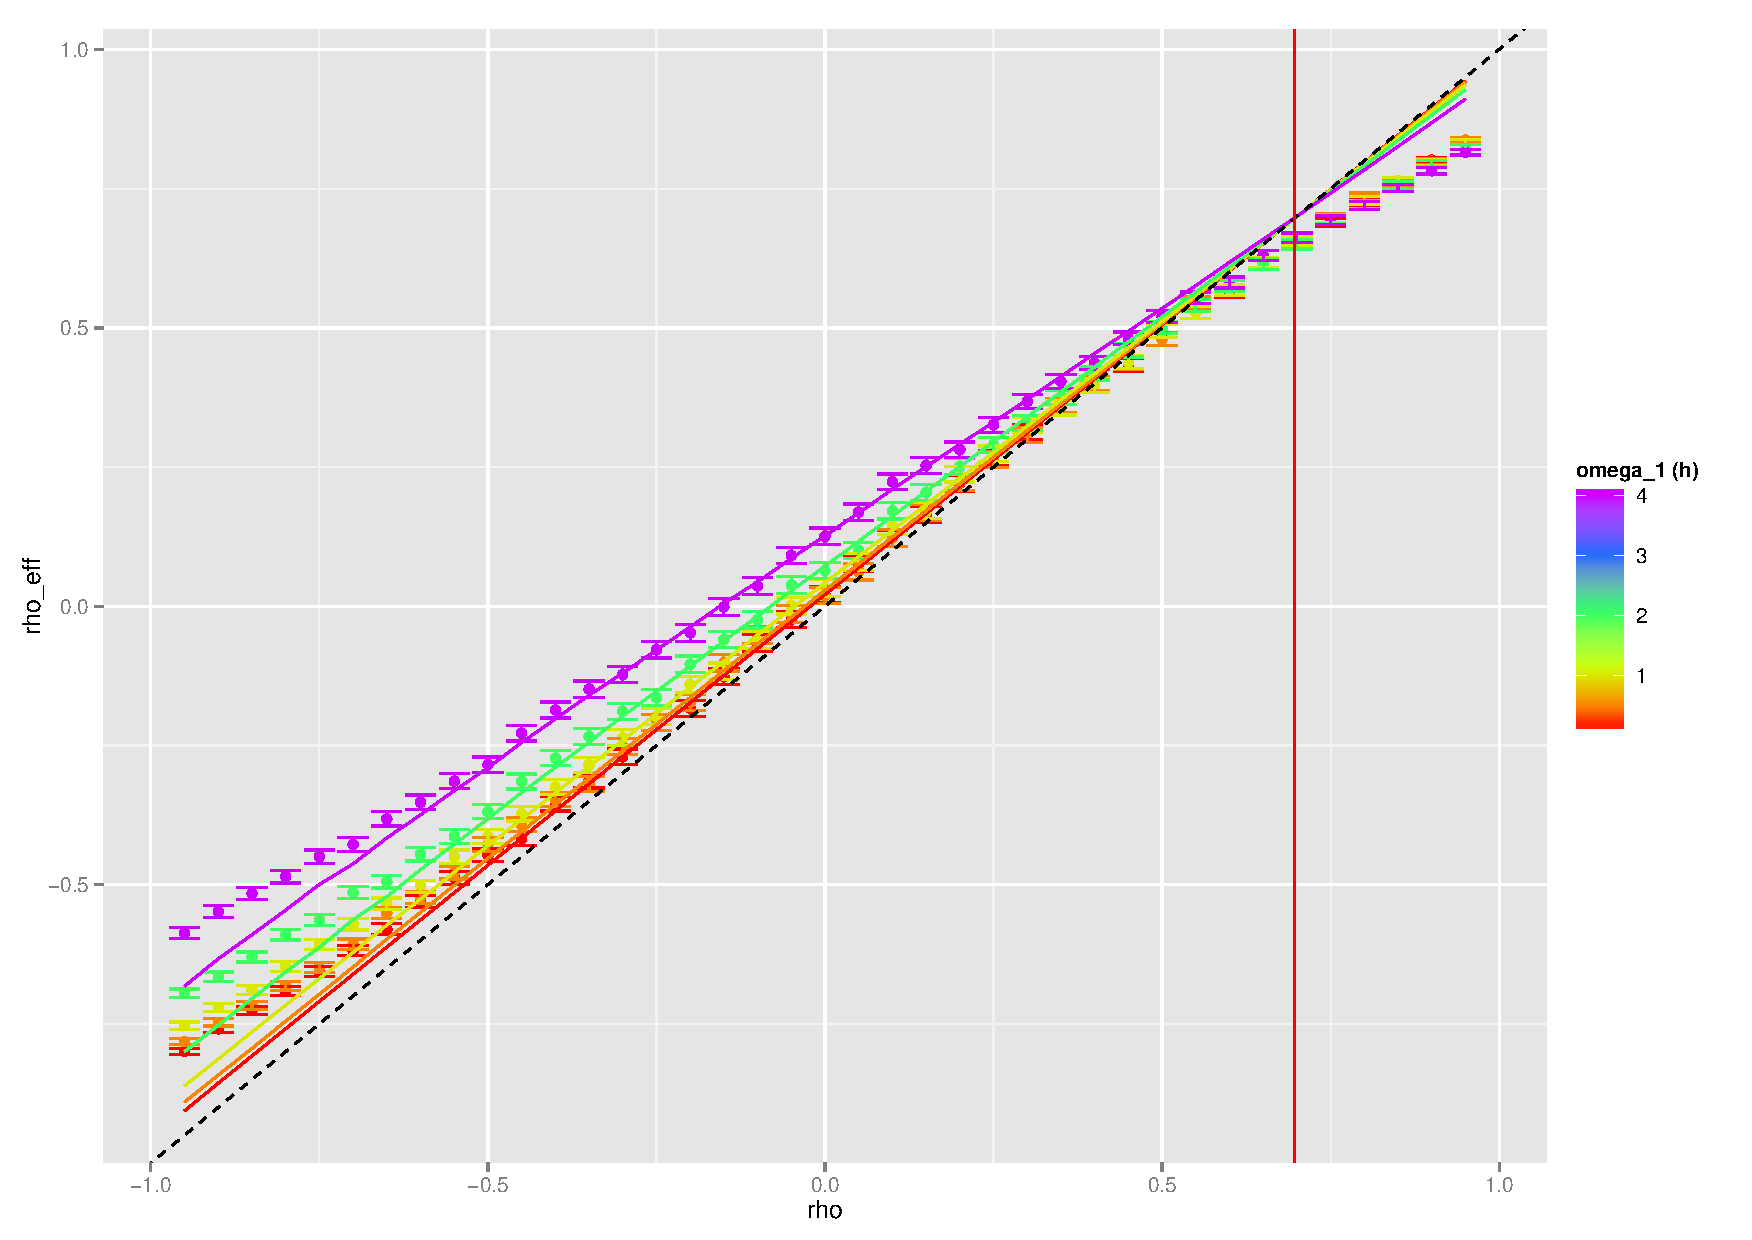
\includegraphics[width=\columnwidth]{figures/effectiveCorrs_withGoodTh_A4}
\caption{\small\textbf{Effective correlations obtained on synthetic data | } Dots represent estimated correlations on a synthetic dataset corresponding to 6 months between June and November 2015 (error-bars give 95\% confidence intervals obtained with standard Fisher method) ; scale color gives filtering frequency $\omega_1=10\textrm{min},30\textrm{min},1\textrm{h},2\textrm{h},4\textrm{h}$ ; solid lines give theoretical values for $\rho_e$ obtained by~\ref{eq:eff_corr} with estimated volatilities (dotted-line diagonal for reference) ; vertical red line position is the theoretical value such that $\rho = \rho_e$ with mean values for $\varepsilon_i$ on all points. We observe for high absolute correlations values a deviation from corrected values, what should be caused by non-verified independence and centered returns assumptions. Asymmetry is caused by the high value of $\rho_0 \simeq 0.71$.}
\label{fig:effective_corrs}
\end{figure}
%%%%%%%%%%%%%%%%%%%


%%%%%%%%%%%%%%%%%%%
\begin{figure*}%[h!]
% figure : performance of arma2 as a function of expected correlation.
%\vspace{-0.7cm}
\centering
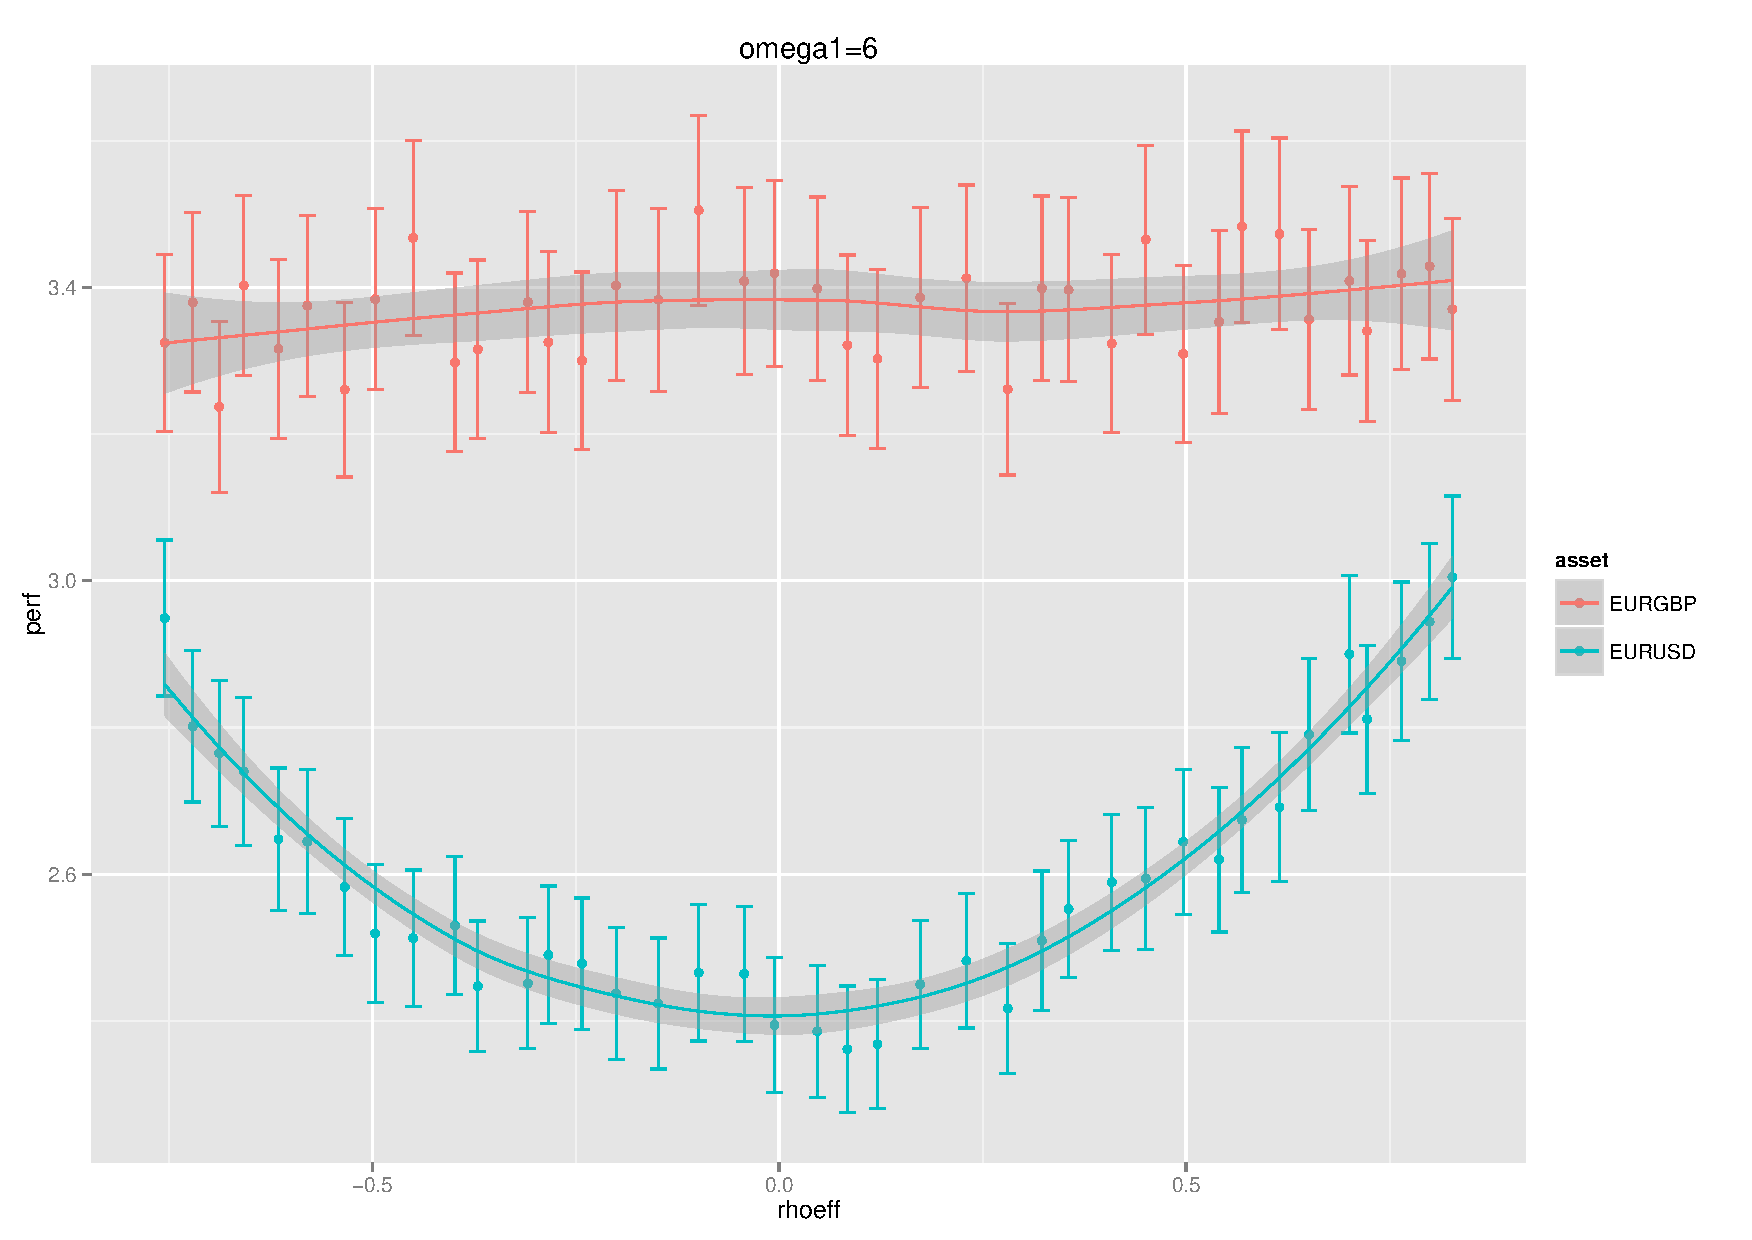
\includegraphics[width=0.48\textwidth]{figures/asset/pred_filt6}
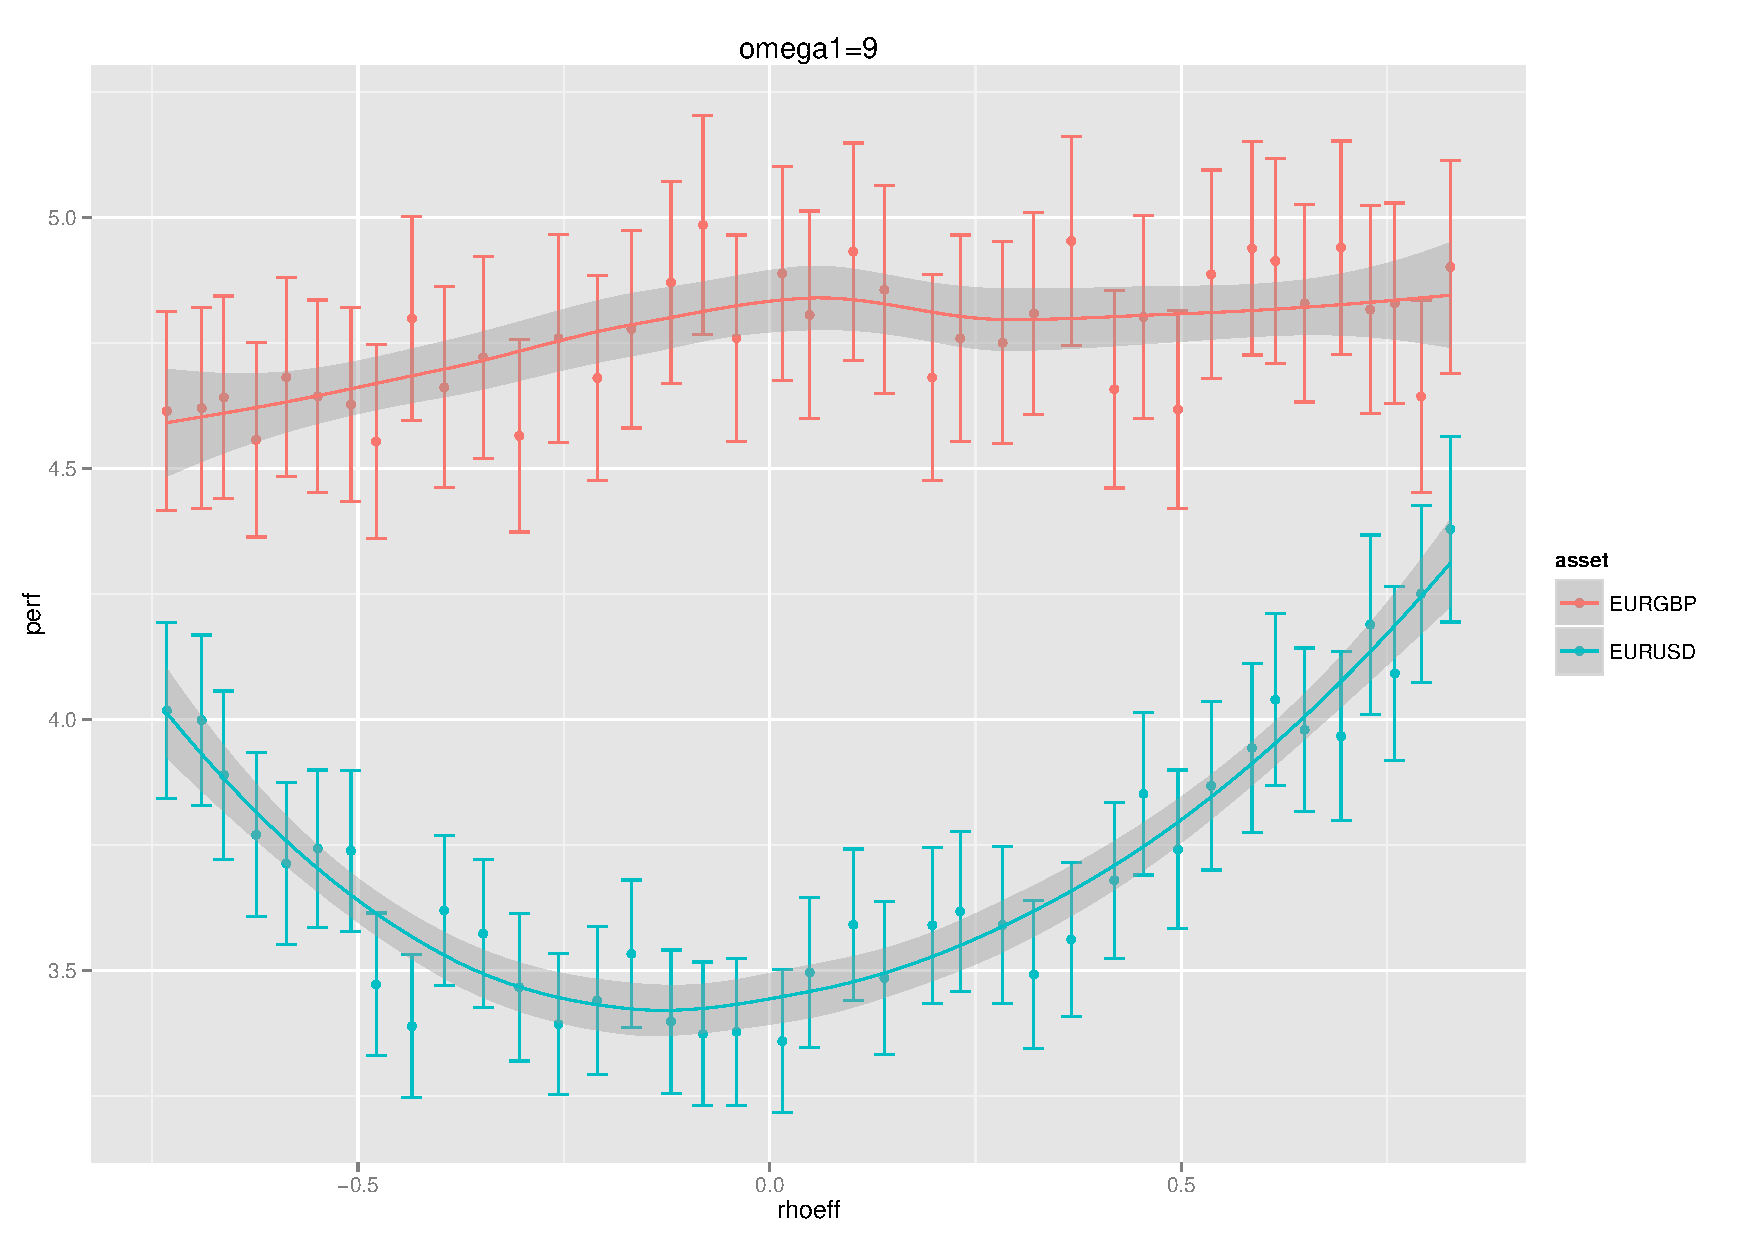
\includegraphics[width=0.48\textwidth]{figures/asset/pred_filt9}\\
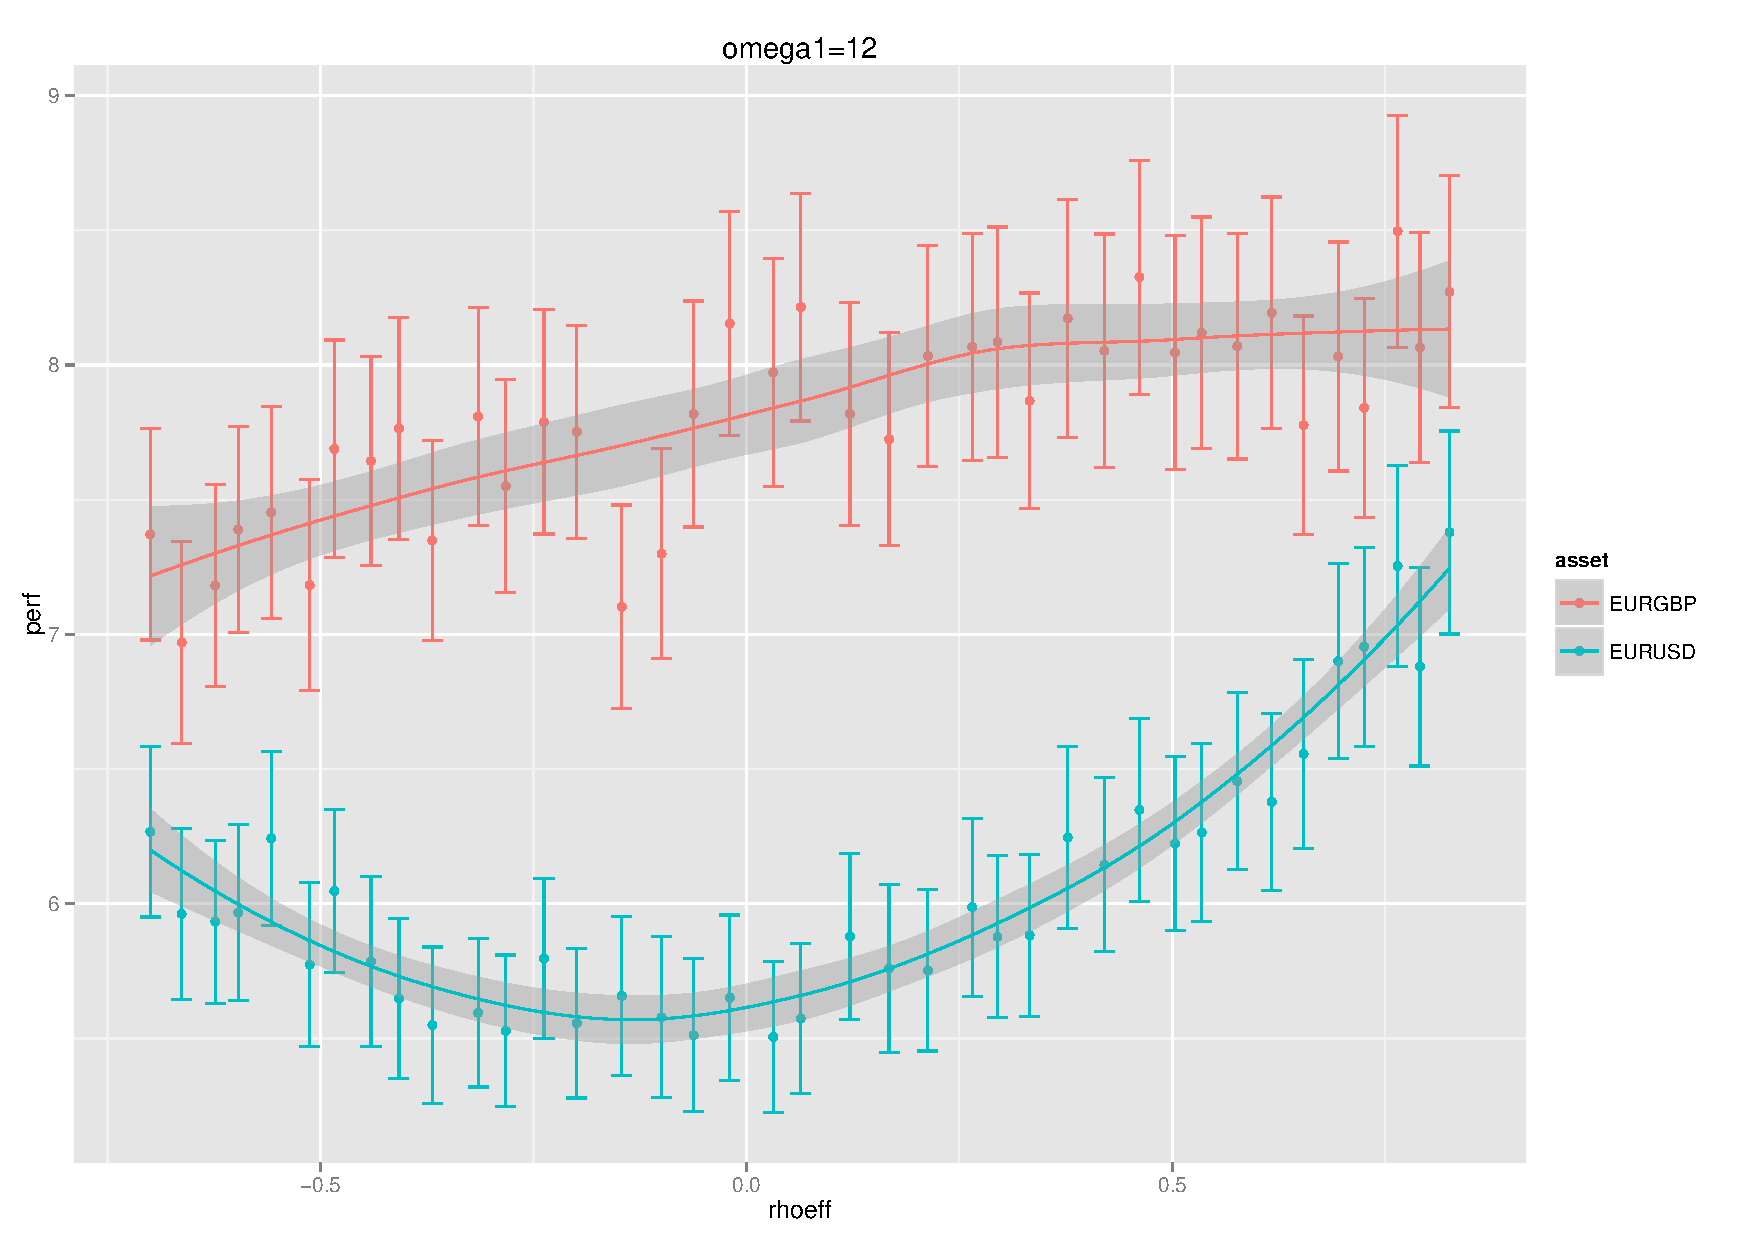
\includegraphics[width=0.48\textwidth]{figures/asset/pred_filt12}
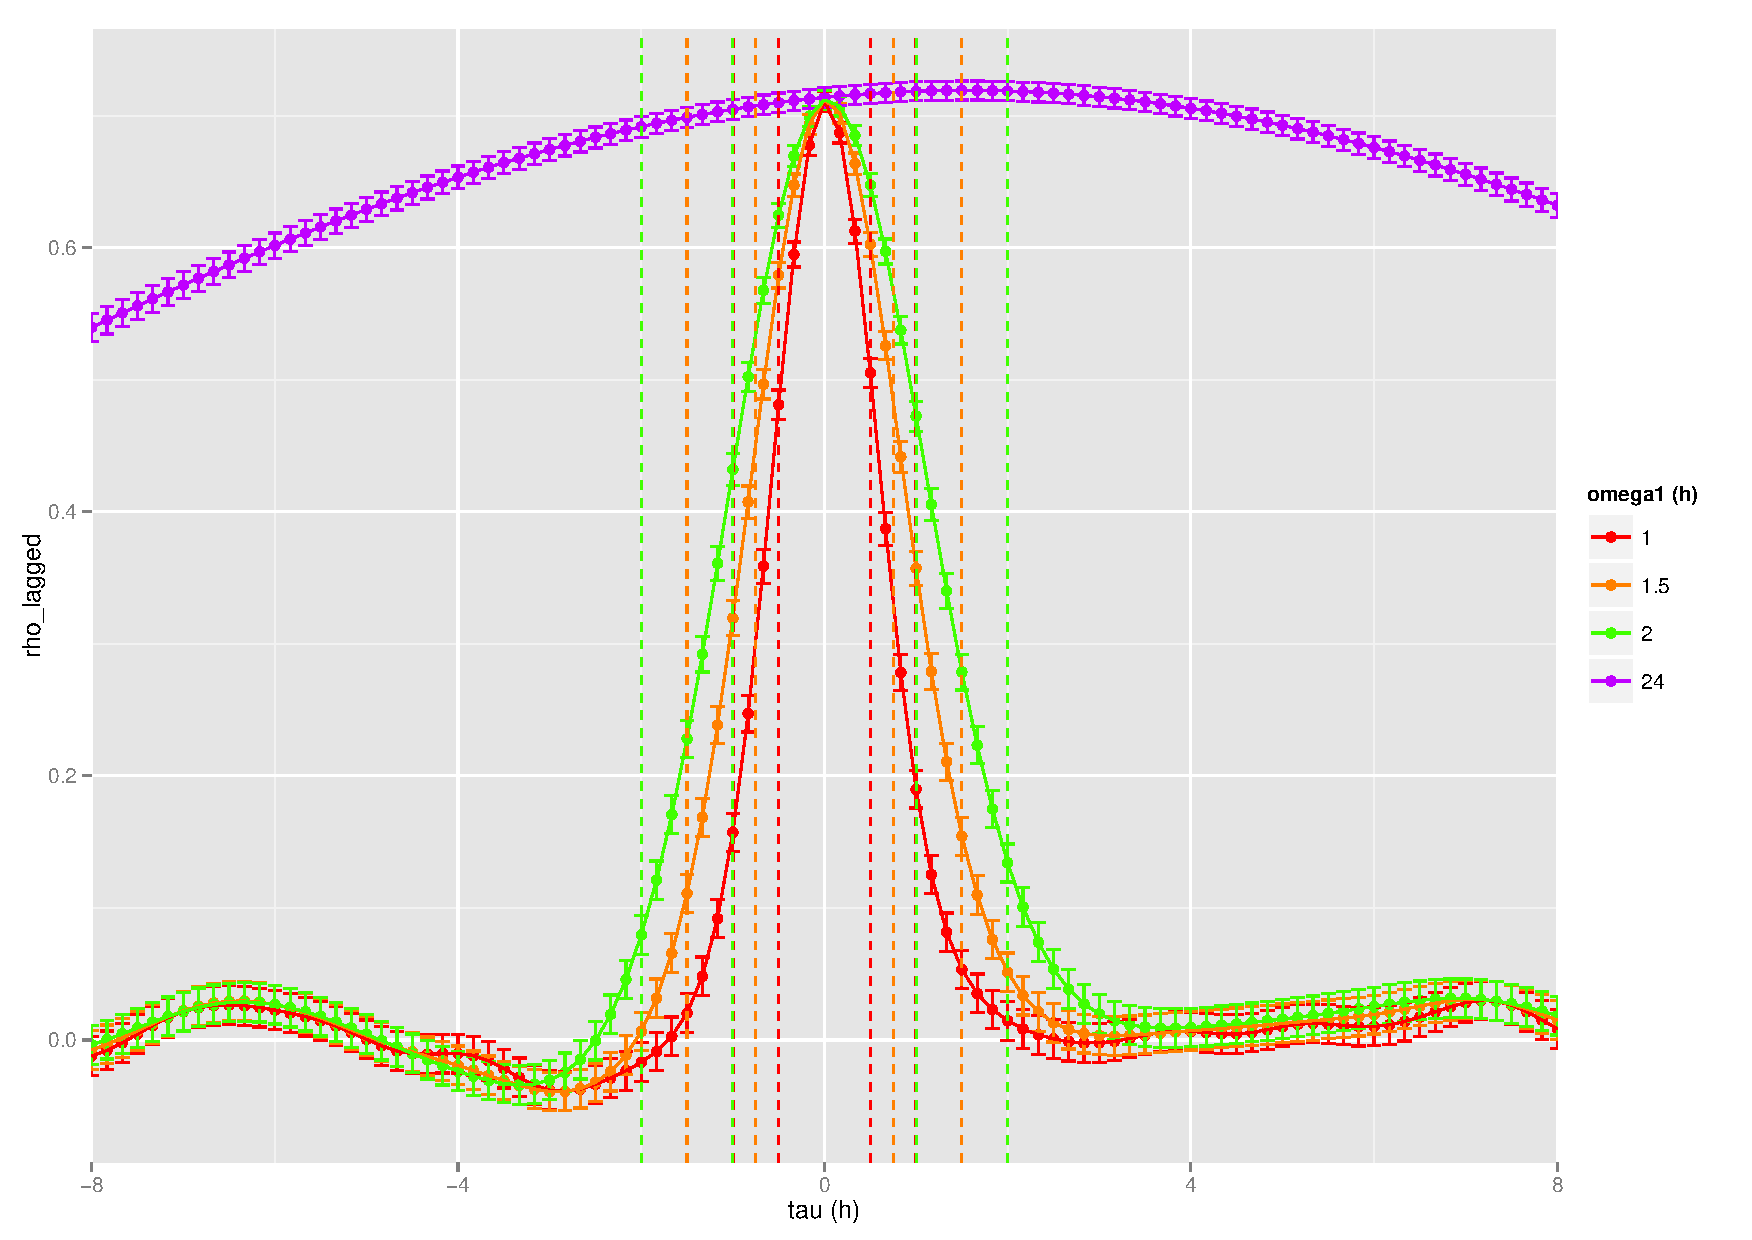
\includegraphics[width=0.48\textwidth]{figures/asset/lagged_corrs}
\caption{\small \textbf{Performance of a predictive model as a function of simulated correlations | } From left to right and top to bottom, three first graphs show for each asset the normalized performance of an ARMA model ($p=2,q=0$), defined as $\pi = \left(\frac{1}{T}\sum_t\left(\tilde{X}_i(t) - M_{\omega_1}\left[\tilde{X}_i\right](t)\right)^2 \right) / \sigma \left[ \tilde{X}_i \right]^2$ (95\% confidence intervals computed by $\pi = \bar{\pi} \pm (1.96\cdot \sigma [\pi])/\sqrt{T}$, local polynomial smoothing to ease reading). It is interesting to note the U-shape for EUR/USD, due to interference between components at different scales. Correlation between simulated noises deteriorates predictive power. The study of \emph{lagged correlations} (here $\rho [\Delta X_{\textrm{EURUSD}}(t),\Delta X_{\textrm{EURGBP}}(t-\tau)]$) on real data clarifies this phenomenon : fourth graph show an asymmetry in curves at any scale compared to zero lag $(\tau = 0)$ what leads fundamental components to increase predictive power for the dollar, amelioration then perturbed by correlations between simulated components. Dashed lines show time steps (in equivalent $\tau$ units) used by the ARMA at each scale, what allows to read the corresponding lagged correlation on fundamental component.}
\label{fig:model_perf}
\end{figure*}
%%%%%%%%%%%%%%%%%%%



\subsection*{Application : geographical data of density and network}


%%%%%%%%%%%%%%%%%%%%%%
\subsubsection{Context}


The use of synthetic data in geography is generally directed towards the generation of synthetic populations within agent-based models (mobility, \emph{LUTI} models)~\cite{pritchard2009advances}. We can make a weak link with some Spatial Analysis techniques. The extrapolation of a continuous spatial field from a discrete spatial sample through a kernel density estimation for example can be understood as the creation of a synthetic dataset (even if it is not generally the initial view, as in Geographically Weighted Regression~\cite{brunsdon1998geographically} in which variable size kernels do not interpolate data \emph{stricto sensu} but extrapolate abstract variables representing interaction between explicit variables). In the field of modeling in quantitative geography, \emph{toy-models} or hybrid models require a consistent initial spatial configuration. A set of possible initial configurations becomes a synthetic dataset on which the model is tested. The first Simpop model~\cite{sanders1997simpop}, precursor of a large family of models later parametrized with real data, could enter that frame but was studied on an unique synthetic spatialization. Similarly underlined was the difficulty to generate an initial transportation infrastructure in the case of the SimpopNet model~\cite{schmitt2014modelisation} although it was admitted as a cornerstone of knowledge on the behavior of the model. A systematic control of spatial configuration effects on the behavior of simulation models was only recently proposed~\cite{cottineau2015revisiting}, approach that can be interpreted as a statistical control on spatial data. The aim is to be able to distinguish proper effects due to intrinsic model dynamics from particular effects due to the geographical structure of the case study. Such results are essential for the validation of conclusions obtained with modeling and simulation practices in quantitative geography.




\subsubsection*{Formalization}

We propose in our case to generate territorial systems summarized in a simplified way as a spatial population density $d(\vec{x})$ and a transportation network $n(\vec{x})$. Correlations we aim to control are correlations between urban morphological measures and network measures. The question of interactions between territories and networks is already well-studied~\cite{offner1996reseaux} but stays highly complex and difficult to quantify~\cite{offner1993effets}. A dynamical modeling of implied processes should shed light on these interactions (\cite{bretagnolle:tel-00459720}, p. 162-163). We develop in that frame a \emph{simple} coupling (i.e. without any feedback loop) between a density distribution model and a network morphogenesis model.




\paragraph{Density model}

We use a model $D$ similar to aggregation-diffusion models~\cite{batty2006hierarchy} to generate a discrete spatial distribution of population density. A generalization of the basic model is proposed in~\cite{raimbault2016calibration}, providing a calibration on morphological objectives (entropy, hierarchy, spatial auto-correlation, mean distance) against real values computed on the set of 50km sized grid extracted from european density grid~\cite{eurostat}. More precisely, the model proceeds iteratively the following way. An square grid of width $N$, initially empty, is represented by population $(P_i(t))_{1\leq i\leq N^2}$. At each time step, until total population reaches a fixed parameter $P_m$,
\begin{itemize}
\item total population is increased of a fixed number $N_G$ (growth rate), following a preferential attachment such that $\Pb{P_i(t+1)=P_i(t)+1|P(t+1)=P(t)+1}=\frac{(P_i(t)/P(t))^{\alpha}}{\sum(P_i(t)/P(t))^{\alpha}}$
\item a fraction $\beta$ of population is diffused to four closest neighbors is operated $n_d$ times
\end{itemize}



The two contradictory processes of urban concentration and urban sprawl are captured by the model, what allows to reproduce with a good precision a large number of existing morphologies.



\paragraph{Network model}


On the other hand, we are able to generate a planar transportation network by a model $N$, at a similar scale and given a density distribution. Because of the conditional nature to the density of the generation process, we will first have conditional estimators for network indicators, and secondly natural correlations between network and urban shapes should appear as processes are not independent. The nature and modularity of these correlations as a function of model parameters are still to determine by exploration of the coupled model.



The heuristic network generation procedure is the following :
\begin{enumerate}
\item A fixed number $N_c$ of centers that will be first nodes of the network si distributed given density distribution, following a similar law to the aggregation process, i.e. the probability to be distributed in a given patch is $\frac{(P_i/P)^{\alpha}}{\sum (P_i/P)^{\alpha}}$. Population is then attributed according to Voronoi areas of centers, such that a center cumulates population of patches within its extent.
\item Centers are connected deterministically by percolation between closest clusters : as soon as network is not connected, two closest connected components in the sense of minimal distance between each vertices are connected by the link realizing this distance. It yields a tree-shaped network.
\item Network is modulated by potential breaking in order to be closer from real network shapes. More precisely, a generalized gravity potential between two centers $i$ and $j$ is defined by
\[
V_{ij}(d) = \left[ (1 - k_h) + k_h \cdot \left( \frac{P_i P_j}{P^2} \right)^{\gamma} \right]\cdot \exp{\left( -\frac{d}{r_g (1 + d/d_0)} \right)}
\]
where $d$ can be euclidian distance $d_{ij}=d(i,j)$ or network distance $d_N(i,j)$, $k_h \in [0,1]$ a weight to modulate role of populations, $\gamma$ giving shape of the hierarchy across population values, $r_g$ characteristic interaction distance and $d_0$ distance shape parameter.
\item A fixed number $K\cdot N_L$ of potential new links is taken among couples having greatest euclidian distance potential ($K=5$ is fixed).
\item Among potential links, $N_L$ are effectively realized, that are the one with smallest rate $\tilde{V}_{ij} = V_{ij}(d_N)/V_{ij}(d_{ij})$. At this stage only the gap between euclidian and network distance is taken into account : $\tilde{V}_{ij}$ does indeed not depend on populations and is increasing with $d_N$ at constant $d_{ij}$.
\item Planarity of the network is forced by creation of nodes at possible intersections created by new links.
\end{enumerate}



We insist on the fact that the network generation procedure is entirely heuristic and result of thematic assumptions (connected initial network, gravity-based link creation) combined with trial-and-error during first explorations. Other model types could be used as well, such biological self-generated networks~\cite{TeroAl10}, local network growth based on geometrical constraints optimization~\cite{barthelemy2008modeling}, or a more complex percolation model than the initial one that would allow the creation of loops for example. We could thus in the frame of a modular architecture, in which the choice between different implementations of a functional brick can be seen as a meta-parameter~\cite{cottineau2015incremental}, choose network generation function adapted to a specific need (as e.g. proximity to real data, constraints on output indicators, variety if generated forms, etc. ).



\paragraph{Parameter space}

Parameter space for the coupled model\footnote{Weak coupling allows to limit the total number of parameters as a strong coupling would involve retroaction loops and consequently associated parameters to determine their structure and intensity. In order to diminish it, an integrated model would be preferable to a strong coupling, what is slightly different in the sense where it is not possible in the integrated model to freeze one of the subsystems to obtain a model of the other subsystem that would correspond to the non-coupled model.} is constituted by density generation parameters $\vec{\alpha}_D = (P_m/N_G , \alpha,\beta , n_d)$ (we study for the sake of simplicity the rate between population and growth rate instead of both varying, i.e. the number of steps needed to generate the distribution) and network generation parameters $\vec{\alpha}_N=(N_C,k_h,\gamma , r_g , d_0)$. We denote $\vec{\alpha} = (\vec{\alpha}_D,\vec{\alpha}_N)$. 



\paragraph{Indicators}

Urban form and network structure are quantified by numerical indicators in order to modulate correlations between these. Morphology is defined as a vector $\vec{M}=(r,\bar{d},\varepsilon,a)$ giving spatial auto-correlation (Moran index), mean distance, entropy and hierarchy (see~\cite{le2015forme} for a precise definition of these indicators). Network measures $\vec{G} = (\bar{c},\bar{l},\bar{s},\delta)$ are with network denoted $(V,E)$
\begin{itemize}
\item Mean centrality $\bar{c}$ defined as average \emph{betweeness-centrality} (normalized in $[0,1]$) on all links.
\item Mean path length $\bar{l}$ given by $\frac{1}{d_m}\frac{2}{|V|\cdot (|V|-1)}\sum_{i<j}d_N(i,j)$ with $d_m$ normalization distance taken here as world diagonal $d_m=\sqrt{2}N$.
\item Mean network speed~\cite{banos2012towards} which corresponds to network performance compared to direct travel, defined as $\bar{s} = \frac{2}{|V|\cdot (|V|-1)}\sum_{i<j}{\frac{d_{ij}}{d_N(i,j)}}$.
\item Network diameter $\delta = \max_{ij}d_N(i,j)$.
\end{itemize}



\paragraph{Covariance and correlation}

We study the cross-correlation matrix $\Covb{\vec{M}}{\vec{G}}$ between morphology and network. We estimate it on a set of $n$ realizations at fixed parameter values $(\vec{M}\left[D(\vec{\alpha})\right],\vec{G}\left[N(\vec{\alpha})\right])_{1\leq i\leq n}$ with standard unbiased estimator. We estimate correlation with associated Pearson estimator. 




%%%%%%%%%%%%%%%%%%%%%%
\subsubsection*{Implementation}


Coupling of generative models is done both at formal and operational levels. We interface therefore independent implementations. The OpenMole software~\cite{reuillon2013openmole} for intensive model exploration offers for that the ideal frame thanks to its modular language allowing to construct \emph{workflows} by task composition and interfacing with diverse experience plans and outputs. For operational reasons, density model is implemented in \texttt{scala} language as an OpenMole \texttt{plugin}, whereas network generation is implemented in agent-oriented language \texttt{NetLogo}~\cite{wilensky1999netlogo} because of its possibilities for interactive exploration and heuristic model construction. Source code is available for reproducibility on project repository\footnote{at \texttt{https://github.com/JusteRaimbault/CityNetwork/tree/master/Models/Synthetic}}.






%%%%%%%%%%%%%%
\begin{figure*}

%\begin{subfigure}[t]{0.35\textwidth}
%\begin{minipage}{0.35\textwidth}
%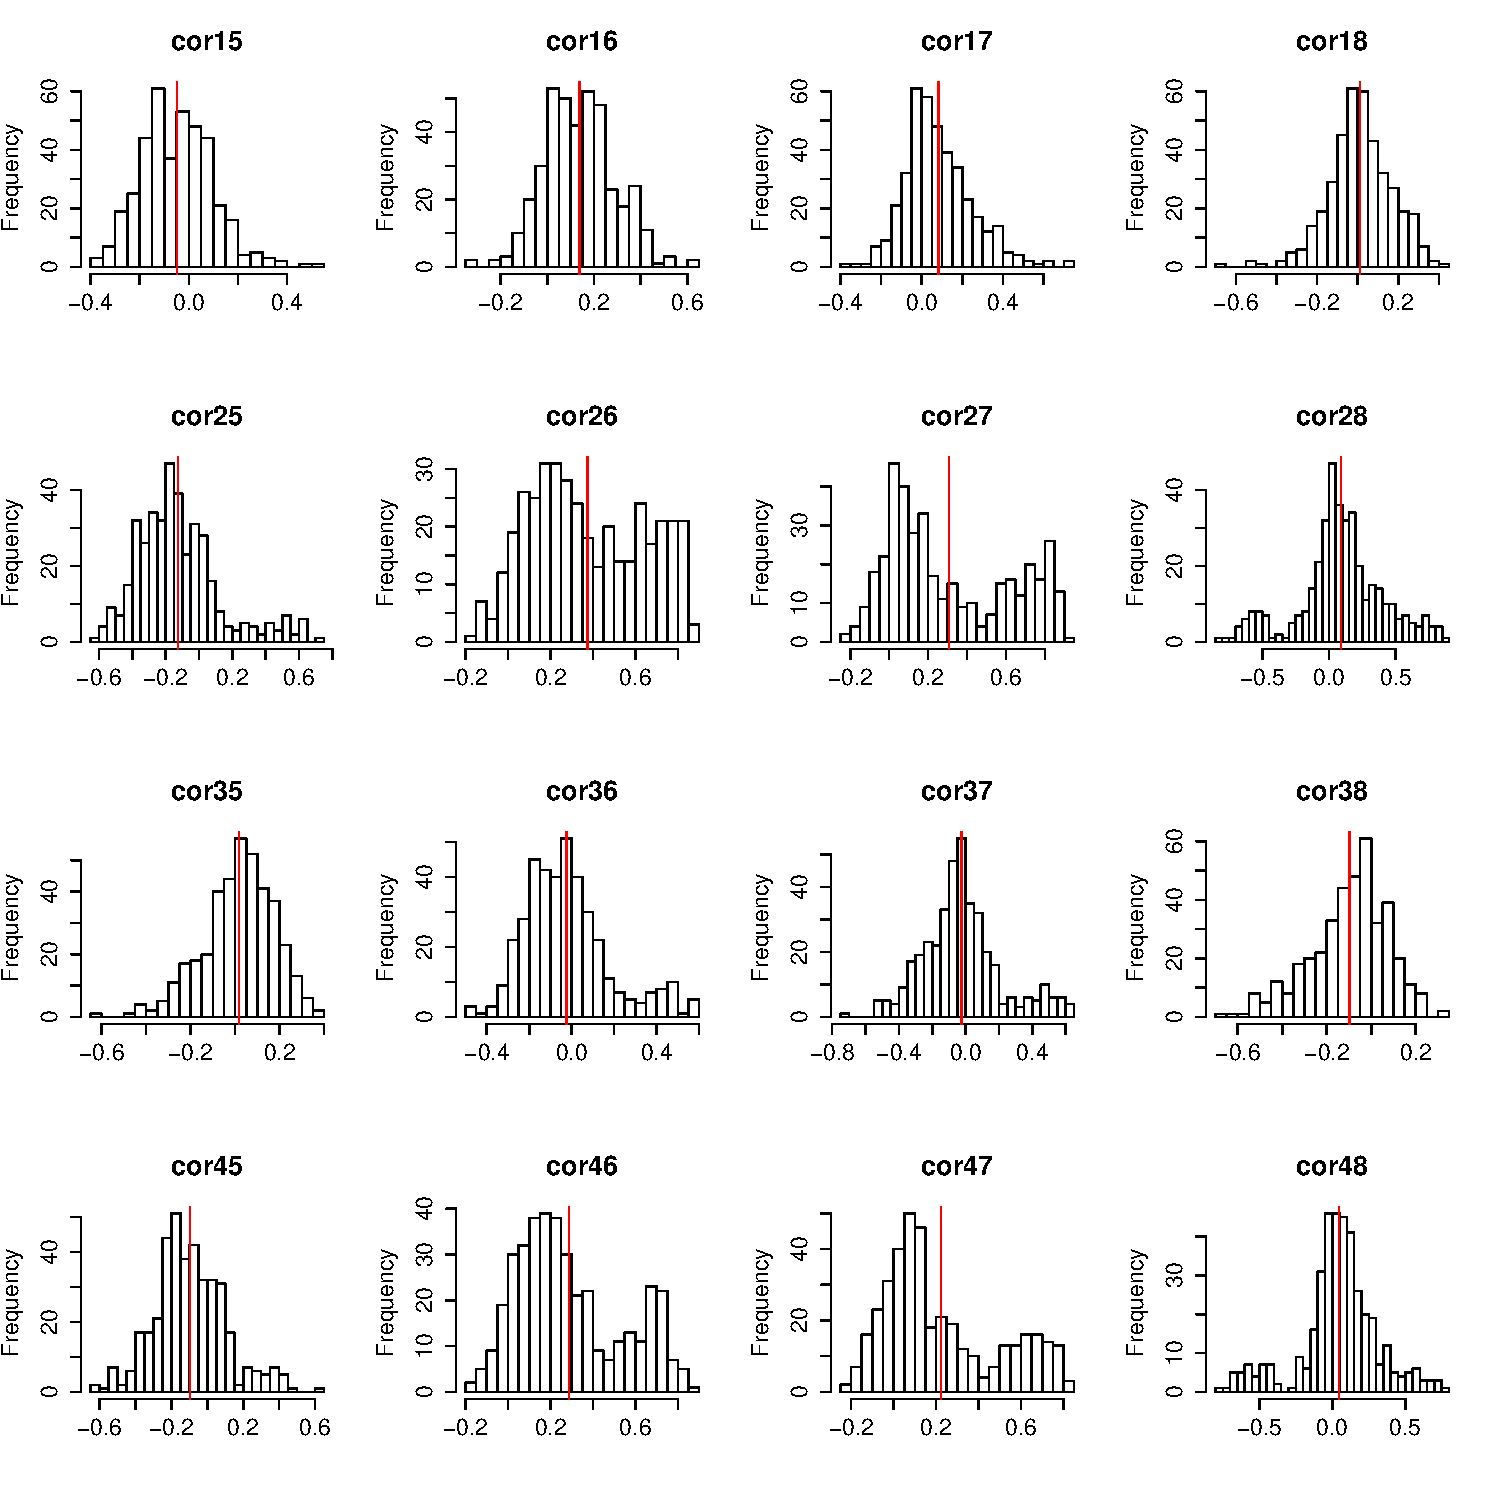
\includegraphics[width=\textwidth]{figures/hist_crossCorMat_breaks30}
%\caption{}
%\end{minipage}
%\end{subfigure}

%\begin{minipage}{0.23\textwidth}
%\vspace{-6.5cm}
%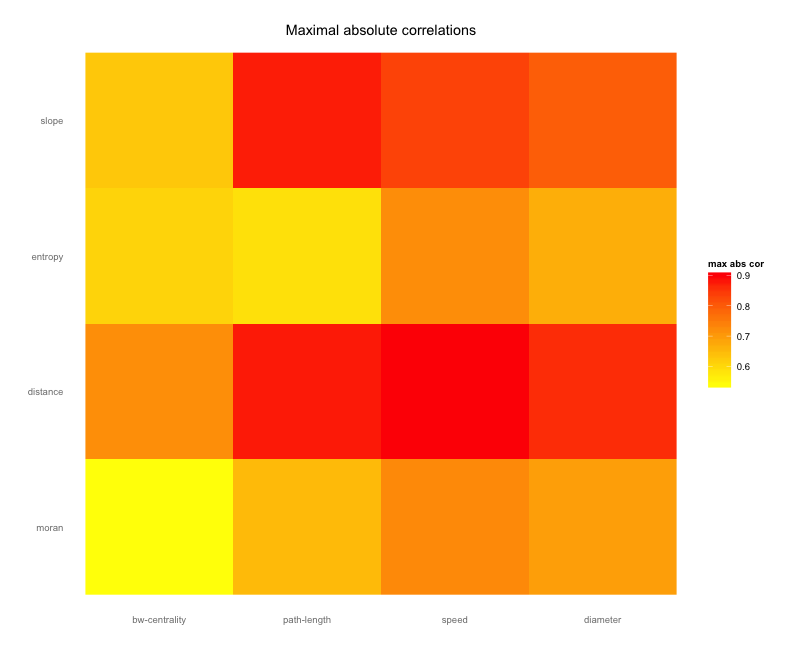
\includegraphics[width=\textwidth]{figures/heatmap_maxAbsCor}\\
%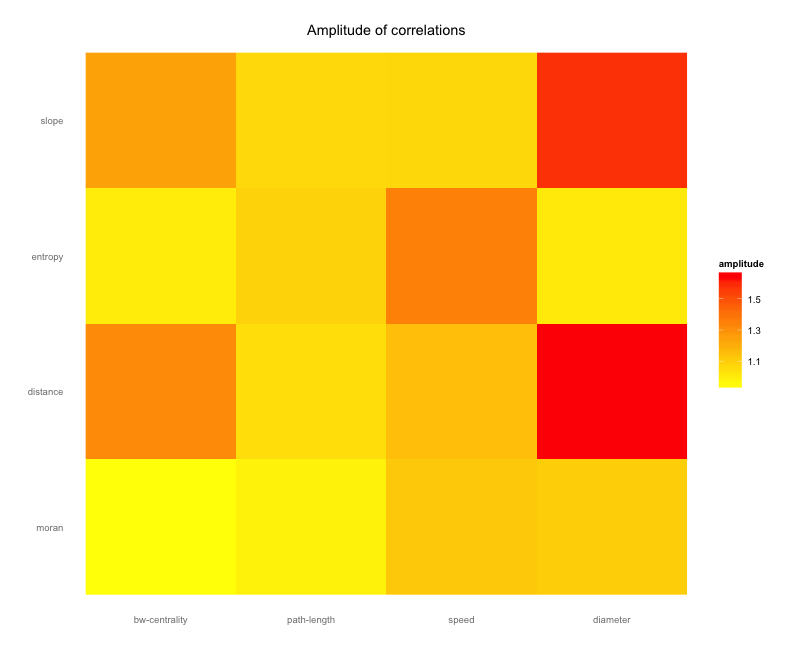
\includegraphics[width=\textwidth]{figures/heatmap_amplCor}
%\caption{}
%\end{minipage}
%\begin{minipage}{0.4\textwidth}
%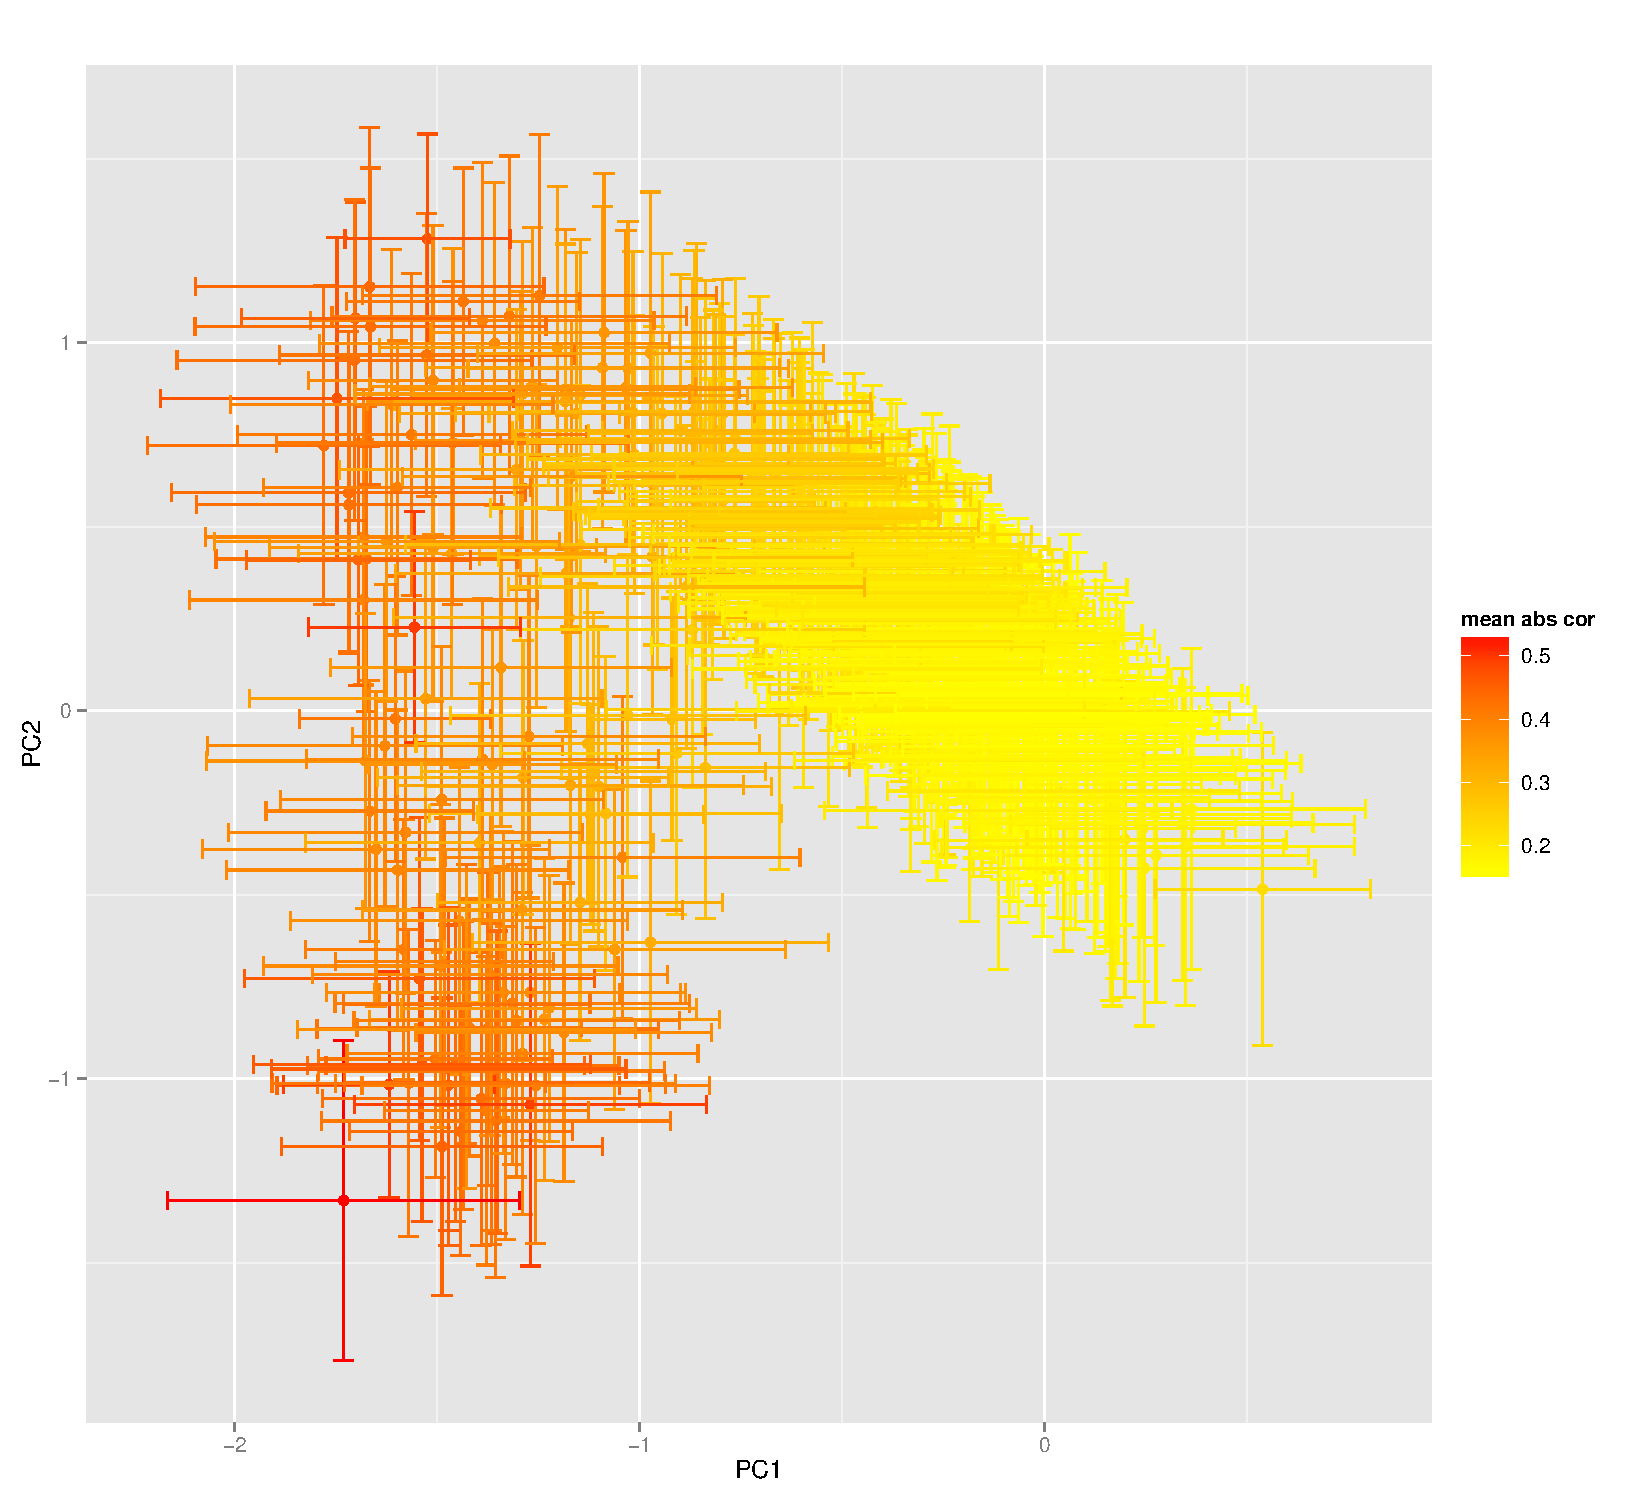
\includegraphics[width=\textwidth]{figures/pca_meanAbsCor_errorBars}
%\caption{}
%\end{minipage}\\
\begin{minipage}{0.54\textwidth}
\vspace{-8.3cm}
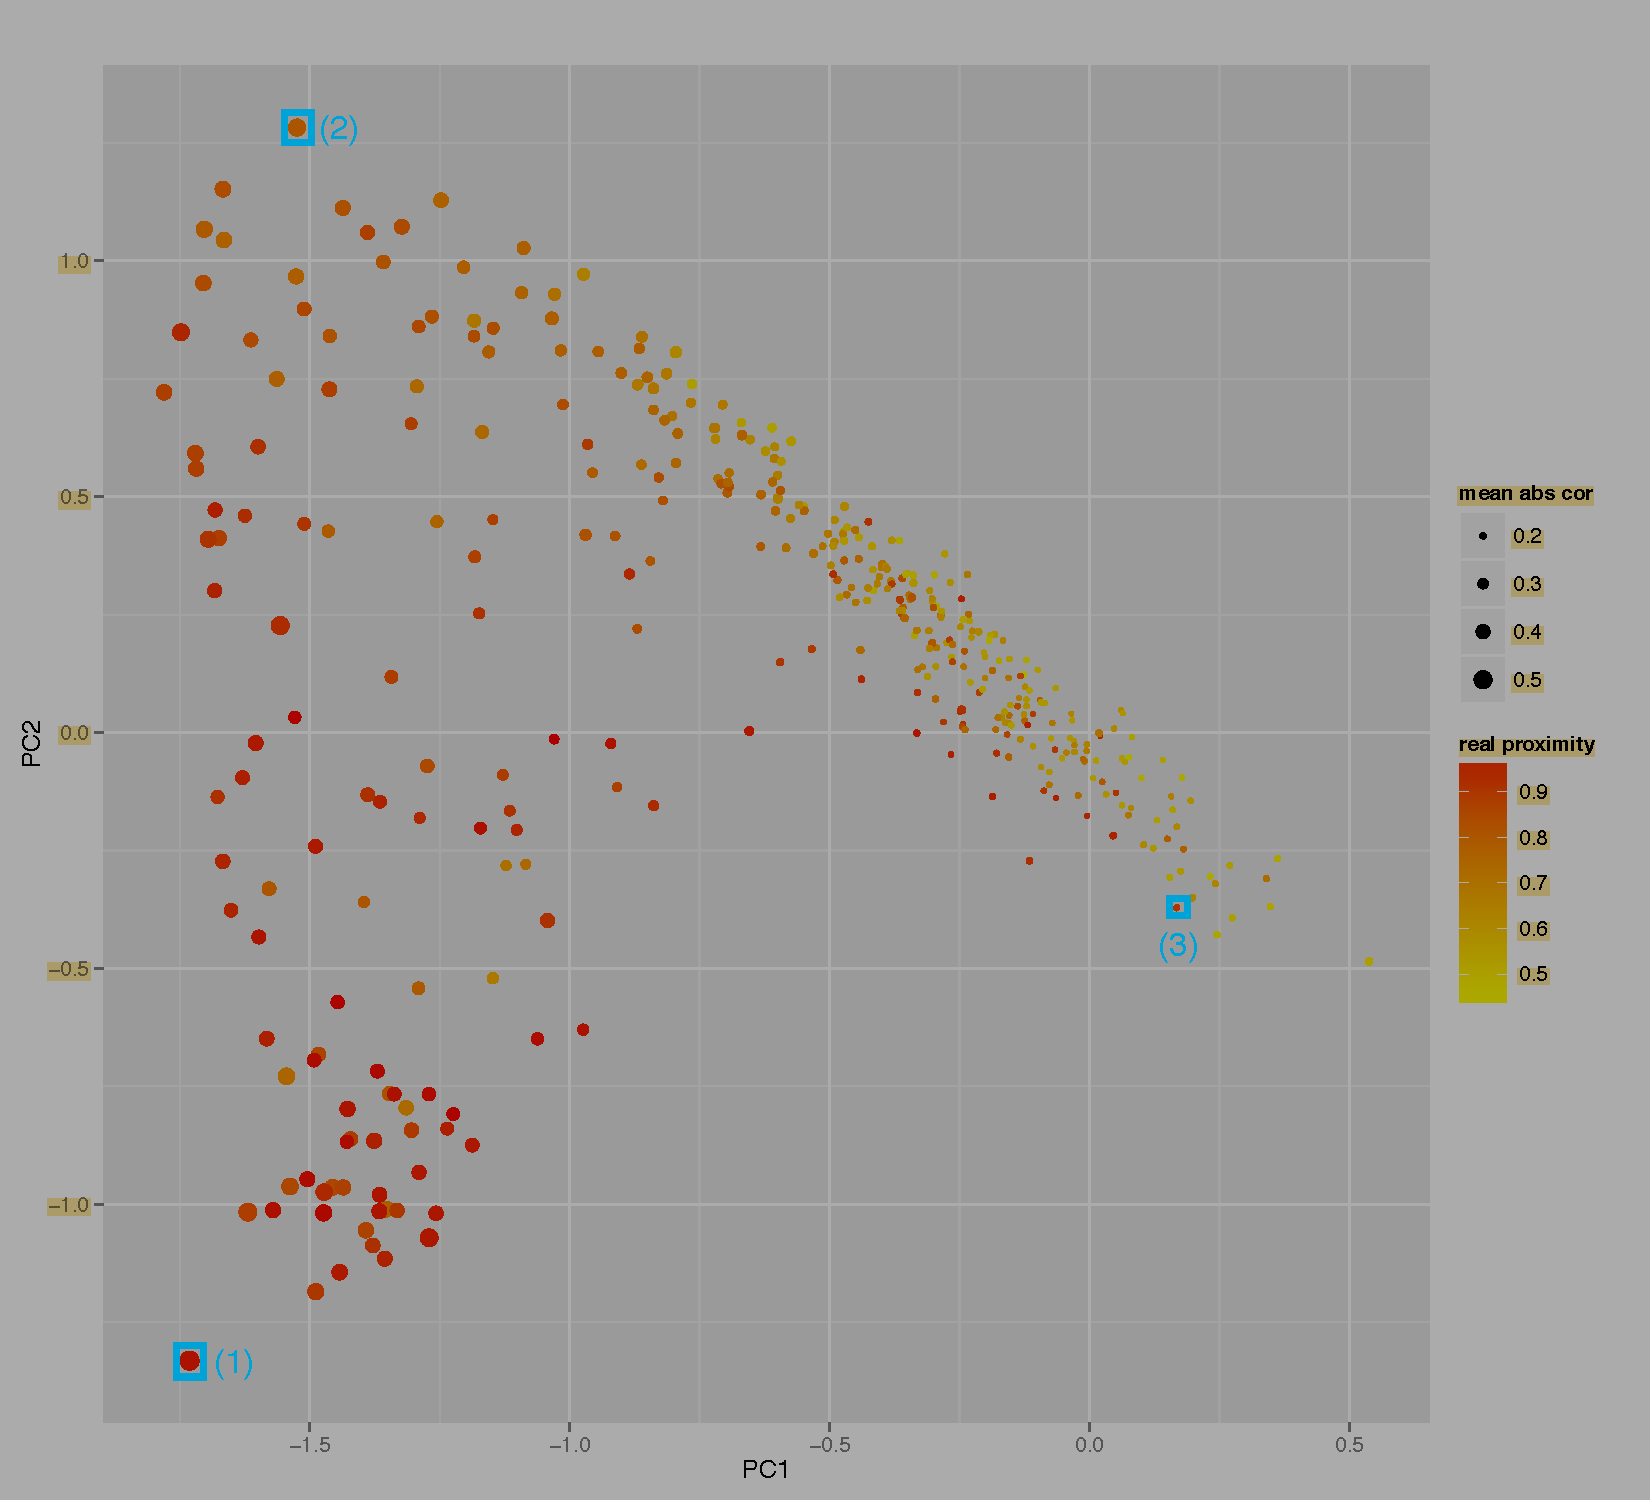
\includegraphics[width=\textwidth]{figures/pca_realDistCol_meanAbsCorSize_withSpecificPoints}
\caption{}
\end{minipage}
\begin{minipage}{0.45\textwidth}
\vspace{-8.3cm}
   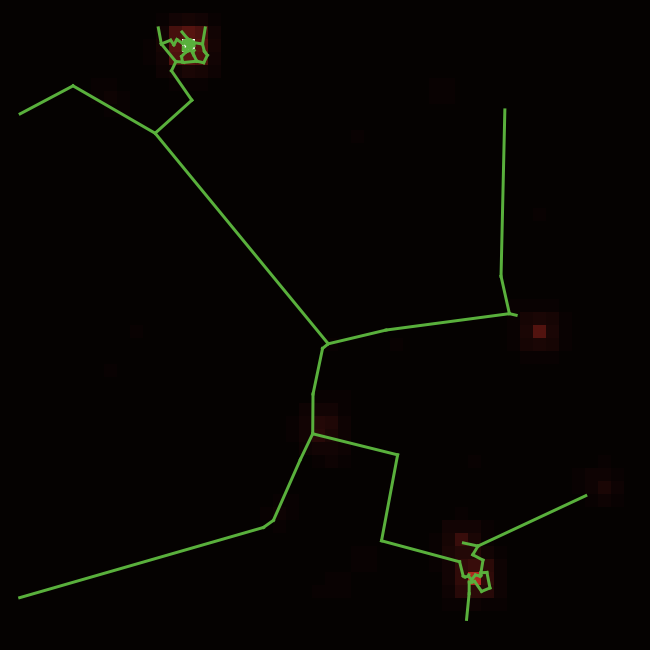
\includegraphics[width=0.49\textwidth]{figures/configs/1_param71861_seed0}
   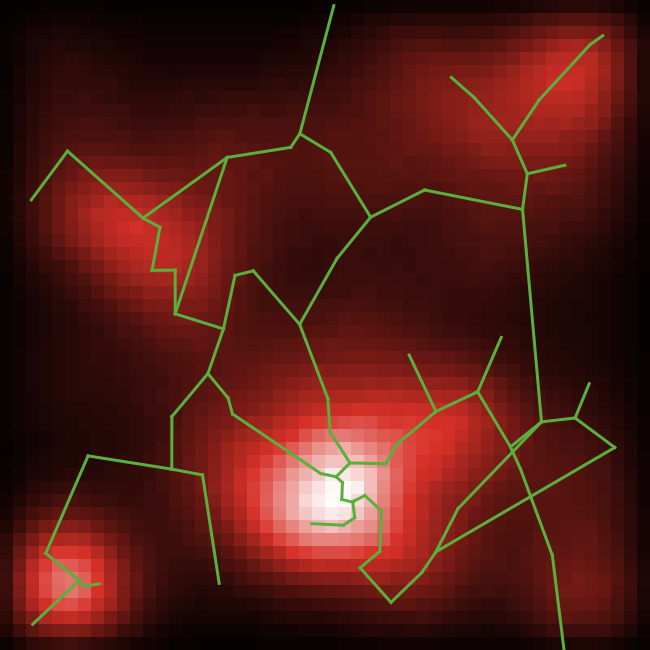
\includegraphics[width=0.49\textwidth]{figures/configs/2_param71913_seed10}\\
   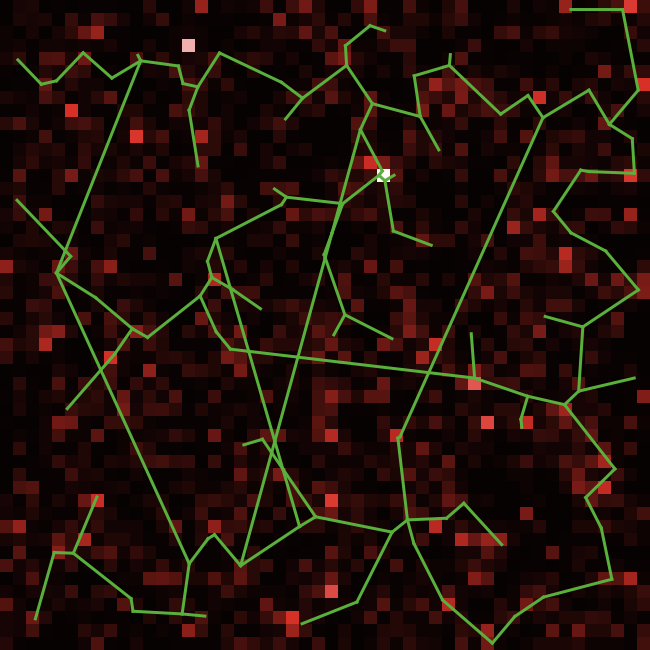
\includegraphics[width=0.49\textwidth]{figures/configs/3_param71918_seed0}
   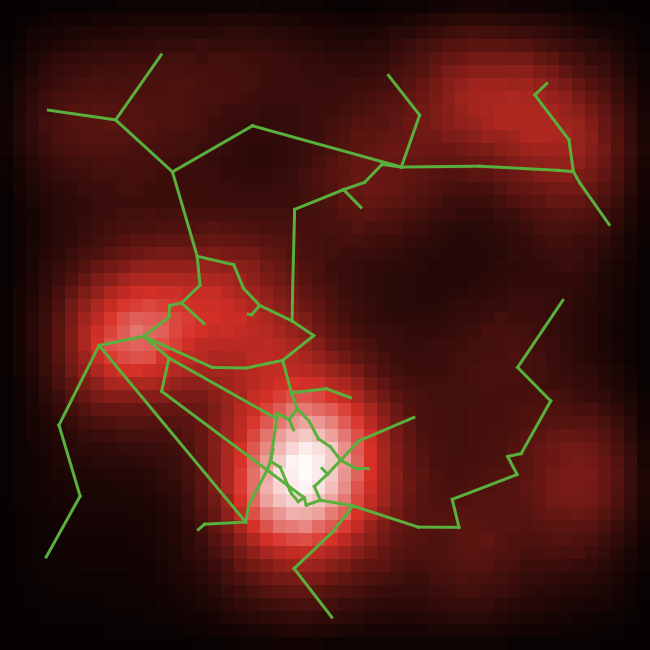
\includegraphics[width=0.49\textwidth]{figures/configs/4_param71945_seed0}
   \caption{}
\end{minipage}

\caption{\small\textbf{Exploration of feasible space for correlations between urban morphology and network structure | } \textbf{(a)} Distribution of crossed-correlations between vectors $\vec{M}$ of morphological indicators (in numbering order moran index, mean distance, entropy, hierarchy) and $\vec{N}$ of network measures (centrality, mean path length, speed, diameter). \textbf{(b)} Heatmaps for amplitude of correlations, defined as $a_{ij}=\max_k{\rho_{ij}^{(k)}}-\min_k{\rho_{ij}^{(k)}}$ and maximal absolute correlation, defined as $c_{ij}=\max_k\left| \rho_{ij}^{k} \right|$. \textbf{(c)} Projection of correlation matrices in a principal plan obtained by Principal Component Analysis on matrix population (cumulated variances: PC1=38\%, PC2=68\%). Error bars are initially computed as 95\% confidence intervals on each matrix element (by standard Fisher asymptotic method), and upper bounds after transformation are taken in principal plan. Scale color gives mean absolute correlation on full matrices. \textbf{(d)} Representation in the principal plan, scale color giving proximity to real data defined as $1 - \min_r \norm{\vec{M}-\vec{M}_r}$ where $\vec{M}_r$ is the set of real morphological measures, point size giving mean absolute correlation. \textbf{(e)} Configurations obtained for parameters giving the four emphasized points in (d), in order from left to right and top to bottom. We recognize polycentric city configurations (2 and 4), diffuse rural settlements (3) and aggregated weak density area (1). See appendice for exhaustive parameter values, indicators and corresponding correlations. For example $\bar{d}$ is highly correlated with $\bar{l},\bar{s}$ ($\simeq$0.8) in (1) but not for (3) although both correspond to rural environments ; in the urban case we observe also a broad variability : $\rho[\bar{d},\bar{c}]\simeq 0.34$ for (4) but $\simeq-0.41$ for (2), what is explained by a stronger role of gravitation hierarchy in (2) $\gamma=3.9,k_h=0.7$ (for (4), $\gamma=1.07,k_h=0.25$), whereas density parameters are similar.}
\label{fig:densnwcor}
\end{figure*}
%%%%%%%%%%%%%%



\subsubsection*{Results}

The study of density model alone is developed in~\cite{raimbault2016calibration}. It is in particular calibrated on European density grid data, on 50km width square areas with 500m resolution for which real indicator values have been computed on whole Europe. Furthermore, a grid exploration of model behavior yields feasible output space in reasonable parameters bounds (roughly $\alpha \in [0.5,2],N_G\in [500,3000], P_m \in [10^4,10^5],\beta\in [0,0.2], n_d \in \{ 1, \ldots , 4\}$). The reduction of indicators space to a two dimensional plan through a Principal Component Analysis (variance explained with two components $\simeq 80\%$) allows to isolate a set of output points that covers reasonably precisely real point cloud. It confirms the ability of the model to reproduce morphologically the set of real configurations.



At given density, the conditional exploration of network generation model parameter space suggest a good flexibility on global indicators $\vec{G}$, together with good convergence properties. For a precise study of model behavior, see appendice giving regressions analysis capturing the behavior of coupled model. In order to illustrate synthetic data generation method, the exploration has been oriented towards the study of cross-correlations.




Given the large relative dimension of parameter space, an exhaustive grid exploration is not possible. We use a Latin Hypercube sampling procedure with bounds given above for $\vec{\alpha}_D$ and for $\vec{\alpha}_N$, we take $N_C \in [50,120], r_g \in [1,100] , d_0 \in [0.1,10] , k_h \in [0,1] , \gamma \in [0.1,4],N_L\in [4,20]$. For number of model replications for each parameter point, less than 50 are enough to obtain confidence intervals at 95\% on indicators of width less than standard deviations. For correlations a hundred give confidence intervals (obtained with Fisher method) of size around 0.4, we take thus $n=80$ for experiments. Figure~\ref{fig:densnwcor} gives details of experiment results. Regarding the subject of correlated synthetic data generation, we can sum up the main lines as following :
\begin{itemize}
\item Empirical distributions of correlation coefficients between morphology and network indicators are not simple and some are bimodal (for example $\rho_{46}=\rho[r,\bar{l}]$  between Moran index and mean path length).
\item it is possible to modulate up to a relatively high level of correlation for all indicators, maximal absolute correlation varying between 0.6 and 0.9. Amplitude of correlations varies between 0.9 and 1.6, allowing a broad spectrum of values. Point cloud in principal plan has a large extent but is not uniform : it is not possible to modulate at will any coefficient as they stay themselves correlated because of underlying generation processes. A more refined study at higher orders (correlation of correlations) would be necessary to precisely understand degrees of freedom in correlation generation.
\item Most correlated points are also the closest to real data, what confirms the intuition and stylized fact of a strong interdependence in reality.
\item Concrete examples taken on particular points in the principal plan show that similar density profiles can yield very different correlation profiles.
\end{itemize}



\subsubsection*{Possible developments}


This case study could be refined by extending correlation control method. A precise knowledge of $N$ behavior (statistical distributions on an exhaustive grid of parameter space) conditional to $D$ would allow to determine $N^{<-1>} | D$ and have more latitude in correlation generation. We could also apply specific exploration algorithms to reach exceptional configurations realizing an expected correlation level, or at least to obtain a better knowledge of the feasible space of correlations~\cite{10.1371/journal.pone.0138212}.





\section*{Discussion}


\subsection*{Scientific positioning}


Our overall approach enters a particular epistemological frame. On the one hand the multidisciplinary aspect, and on the other hand the importance of empirical component through computational exploration methods, make this approach typical of Complex Systems science, as it is recalled by the roadmap for Complex Systems having a similar structure~\cite{2009arXiv0907.2221B}. It combines transversal research questions (horizontal integration of disciplines) with the development of heterogeneous multi-scalar approaches which encounter similar issues as the one we proposed to tackle (vertically integrated disciplines). The combination of empirical knowledge obtained from data mining, with knowledge obtained by modeling and simulation is generally central to the conception and exploration of multi-scalar heterogeneous models. Results presented here is an illustration of such an hybrid paradigm.



\subsection*{Direct applications}


Starting from the second example which was limited to data generation, we propose examples of direct applications that should give an overview of the range of possibilities.


\begin{itemize}
\item Calibration of network generation component at given density, on real data for transportation network (typically road network given the shape of generated networks ; it should be straightforward to use OpenStreetMap open data\footnote{\texttt{https://www.openstreetmap.org}} that have a reasonable quality for Europe, at least for France~\cite{girres2010quality}, with however adjustments on generation procedure in order to avoid edge effects due its restrictive frame, for example by generating on an extended surface to keep only a central area on which calibration would be done) should theoretically allow to unveil parameter sets reproducing accurately existing configurations both for urban morphology and network shape. It could be then possible to derive a ``theoretical correlation'' for these, as an empirical correlation is according to some theories of urban systems not computable as a unique realization of stochastic processes is observed. Because of non-ergodicity of urban systems~\cite{pumain2012urban}, there are strong chances that involved processes are different across different geographical areas (or from an other point of view that they are in an other state of meta-parameters, i.e. in an other regime) and that their interpretation as different realizations of the same stochastic process makes no sense, the impossibility of covariation estimation following. By attributing a synthetic dataset similar to a given real configuration, we would be able to compute a sort of \emph{intrinsic correlation} proper to this configuration. As territorial configurations emerge from spatio-temporal interdependences between components of territorial systems, this intrinsic correlation emerges the same way, and its knowledge gives information on these interdependences and thus on relations between territories and networks.
\item As already mentioned, most of models of simulation need an initial state generated artificially as soon as model parametrization is not done completely on real data. An advanced model sensitivity analysis implies a control on parameters for synthetic dataset generation, seen as model meta-parameters~\cite{cottineau2015revisiting}. In the case of a statistical analysis of model outputs it provides a way to operate a second order statistical control.
\item We studied in the first example stochastic processes in the sense of random time-series, whereas time did not have a role in the second case. We can suggest a strong coupling between the two model components (or the construction of an integrated model) and to observe indicators and correlations at different time steps during the generation. In a dynamical spatial models we have because of feedbacks necessarily propagation effects and therefore the existence of lagged interdependences in space and time~\cite{pigozzi1980interurban}. It would drive our field of study towards a better understanding of dynamical correlations.
\end{itemize}




\subsection*{Generalization}

We were limited to the control of first and second moments of generated data, but we could imagine a theoretical generalization allowing the control of moments at any order. However, as shown by the geographical example, the difficulty of generation in a concrete complex case questions the possibility of higher orders control when keeping a consistent structure model and a reasonable number of parameters. The study of non-linear dependence structures as proposed in~\cite{chicheportiche2013nested} is in an other perspective an interesting possible development.






\section*{Conclusion}


We proposed an abstract method to generate synthetic datasets in which correlation structure is controlled. Its rapid implementation in two very different fields shows its flexibility and the broad range of possible applications. More generally, it is crucial to favorise such practices of systematic validation of computational models by statistical analysis, in particular for agent-based models for which the question of validation stays an open issue.






%
%\subsection*{Author Affiliations}
%
%Include department, institution, and complete address, with the ZIP/postal code, for each author. Use lower case letters to match authors with institutions, as shown in the example. Authors with an ORCID ID may supply this information at submission.
%
%\subsection*{Format}
%
%Many authors find it useful to organize their manuscripts with the following order of sections;  Title, Author Affiliation, Keywords, Abstract, Significance Statement, Results, Discussion, Materials and methods, Acknowledgments, and References. Other orders and headings are permitted.
%
%\subsection*{Manuscript Length}
%
%PNAS generally uses a two-column format averaging 67 characters, including spaces, per line. The maximum length of a Direct Submission research article is six pages and a PNAS PLUS research article is ten pages including all text, spaces, and the number of characters displaced by figures, tables, and equations.  When submitting tables, figures, and/or equations in addition to text, keep the text for your manuscript under 39,000 characters (including spaces) for Direct Submissions and 72,000 characters (including spaces) for PNAS PLUS.
%
%\subsection*{References}
%
%References should be cited in numerical order as they appear in text; this will be done automatically via bibtex, e.g. \cite{belkin2002using} and \cite{berard1994embedding,coifman2005geometric}. All references, including for the SI, should be included in the main manuscript file. References appearing in both sections should not be duplicated.  SI references included in tables should be included with the main reference section. 
%
%\subsection*{Data Archival}
%
%PNAS must be able to archive the data essential to a published article. Where such archiving is not possible, deposition of data in public databases, such as GenBank, ArrayExpress, Protein Data Bank, Unidata, and others outlined in the Information for Authors, is acceptable.
%
%\subsection*{Language-Editing Services}
%Prior to submission, authors who believe their manuscripts would benefit from professional editing are encouraged to use a language-editing service (see list at www.pnas.org/site/authors/language-editing.xhtml). PNAS does not take responsibility for or endorse these services, and their use has no bearing on acceptance of a manuscript for publication. 
%
%\begin{figure}%[tbhp]
%\centering
%\includegraphics[width=.8\linewidth]{frog}
%\caption{Placeholder image of a frog with a long example caption to show justification setting.}
%\label{fig:frog}
%\end{figure}
%
%\subsection*{Digital Figures}
%\label{sec:figures}
%
%Only TIFF, EPS, and high-resolution PDF for Mac or PC are allowed for figures that will appear in the main text, and images must be final size. Authors may submit U3D or PRC files for 3D images; these must be accompanied by 2D representations in TIFF, EPS, or high-resolution PDF format.  Color images must be in RGB (red, green, blue) mode. Include the font files for any text. 
%
%Figures and Tables should be labelled and referenced in the standard way using the \verb|\label{}| and \verb|\ref{}| commands.
%
%Figure \ref{fig:frog} shows an example of how to insert a column-wide figure. To insert a figure wider than one column, please use the \verb|\begin{figure*}...\end{figure*}| environment. Figures wider than one column should be sized to 11.4 cm or 17.8 cm wide.
%
%\subsection*{Single column equations}
%
%Authors may use 1- or 2-column equations in their article, according to their preference.
%
%To allow an equation to span both columns, options are to use the \verb|\begin{figure*}...\end{figure*}| environment mentioned above for figures, or to use the \verb|\begin{widetext}...\end{widetext}| environment as shown in equation \ref{eqn:example} below.
%
%Please note that this option may run into problems with floats and footnotes, as mentioned in the \href{http://texdoc.net/pkg/cuted}{cuted package documentation}. In the case of problems with footnotes, it may be possible to correct the situation using commands \verb|\footnotemark| and \verb|\footnotetext|.
%
%%% Do not use widetext if paper is in single column.
%\begin{widetext}
%\begin{align*}
%(x+y)^3&=(x+y)(x+y)^2\\
%       &=(x+y)(x^2+2xy+y^2) \numberthis \label{eqn:example} \\
%       &=x^3+3x^2y+3xy^3+x^3. 
%\end{align*}
%\end{widetext}
%
%\begin{table}%[tbhp]
%\centering
%\caption{Comparison of the fitted potential energy surfaces and ab initio benchmark electronic energy calculations}
%\begin{tabular}{lrrr}
%Species & CBS & CV & G3 \\
%\midrule
%1. Acetaldehyde & 0.0 & 0.0 & 0.0 \\
%2. Vinyl alcohol & 9.1 & 9.6 & 13.5 \\
%3. Hydroxyethylidene & 50.8 & 51.2 & 54.0\\
%\bottomrule
%\end{tabular}
%
%\addtabletext{nomenclature for the TSs refers to the numbered species in the table.}
%\end{table}
%
%\subsection*{Supporting Information (SI)}
%
%The main text of the paper must stand on its own without the SI. Refer to SI in the manuscript at an appropriate point in the text. Number supporting figures and tables starting with S1, S2, etc. Authors are limited to no more than 10 SI files, not including movie files. Authors who place detailed materials and methods in SI must provide sufficient detail in the main text methods to enable a reader to follow the logic of the procedures and results and also must reference the online methods. If a paper is fundamentally a study of a new method or technique, then the methods must be described completely in the main text. Because PNAS edits SI and composes it into a single PDF, authors must provide the following file formats only.
%
%\subsubsection*{SI Text}
%
%Supply Word, RTF, or LaTeX files (LaTeX files must be accompanied by a PDF with the same file name for visual reference).
%
%\subsubsection*{SI Figures}
%
%Provide a brief legend for each supporting figure after the supporting text. Provide figure images in TIFF, EPS, high-resolution PDF, JPEG, or GIF format; figures may not be embedded in manuscript text. When saving TIFF files, use only LZW compression; do not use JPEG compression. Do not save figure numbers, legends, or author names as part of the image. Composite figures must be pre-assembled.
%
%\subsubsection*{3D Figures}
%
%Supply a composable U3D or PRC file so that it may be edited and composed. Authors may submit a PDF file but please note it will be published in raw format and will not be edited or composed.
%
%\subsubsection*{SI Tables}
%
%Supply Word, RTF, or LaTeX files (LaTeX files must be accompanied by a PDF with the same file name for visual reference); include only one table per file. Do not use tabs or spaces to separate columns in Word tables.
%
%\subsubsection*{SI Datasets} 
%
%Supply Excel (.xls), RTF, or PDF files. This file type will be published in raw format and will not be edited or composed. 
%
%\subsubsection*{SI Movies}
%
%Supply Audio Video Interleave (avi), Quicktime (mov), Windows Media (wmv), animated GIF (gif), or MPEG files and submit a brief legend for each movie in a Word or RTF file. All movies should be submitted at the desired reproduction size and length. Movies should be no more than 10 MB in size. 
%
%\subsubsection*{Still images}
%
%Authors must provide a still image from each video file. Supply TIFF, EPS, high-resolution PDF, JPEG, or GIF files. 
%
%\subsubsection*{Appendices}
%
%PNAS prefers that authors submit individual source files to ensure readability. If this is not possible, supply a single PDF file that contains all of the SI associated with the paper. This file type will be published in raw format and will not be edited or composed.
%
\matmethods{
%Please describe your materials and methods here. This can be more than one paragraph, and may contain subsections and equations as required. Authors should include a statement in the methods section describing how readers will be able to access the data in the paper. 
%
%\subsection*{Subsection for Method}
%Example text for subsection.




\paragraph{Methodology}

The method is tested on an example with two assets from foreign exchange market (EUR/USD and EUR/GBP), in a six month period from June 2015 to November 2015. Data\footnote{obtained from \texttt{http://www.histdata.com/}, without specified licence. For the respect of copyright, only cleaned and filtered at $\omega_m$ data are made openly available.} cleaning, starting from original series sampled at a frequency around 1s, consists in a first step to the determination of the minimal common temporal range (missing sequences being ignored, by vertical translation of series, i.e. $S(t):=S(t)\cdot \frac{S(t_{n})}{S(t_{n-1})}$ when $t_{n-1},t_n$ are extremities of the ``hole'' and $S(t)$ value of the asset, what is equivalent to keep the constraint to have returns at similar temporal steps between assets). We study then \emph{log-prices} and \emph{log-returns}, defined by $X(t):=\log{\frac{S(t)}{S_0}}$ and $\Delta X (t) = X(t) - X(t-1)$. Raw data are filtered at a maximal frequency $\omega_m = 10\textrm{min}$ (which will be the maximal frequency for following treatments) for concerns of computational efficiency\footnote{as time-series are then sampled at $3\cdot\omega_m$ to avoid aliasing, a day of size 86400 for 1s sampling is reduced to a much smaller size of 432.}. We use a non-causal gaussian filter of total width $\omega$. We fix the fundamental frequency $\omega_0=24\textrm{h}$ and we propose to construct synthetic data at frequencies $\omega_1 = 30\textrm{min},1\textrm{h},2\textrm{h}$. 
%See Fig.~\ref{fig:example_signal} for an example of signal structure at these different scales.


%%%%%%%%%%%%%%%%%%%
%\begin{figure}%[h!]
%\centering
%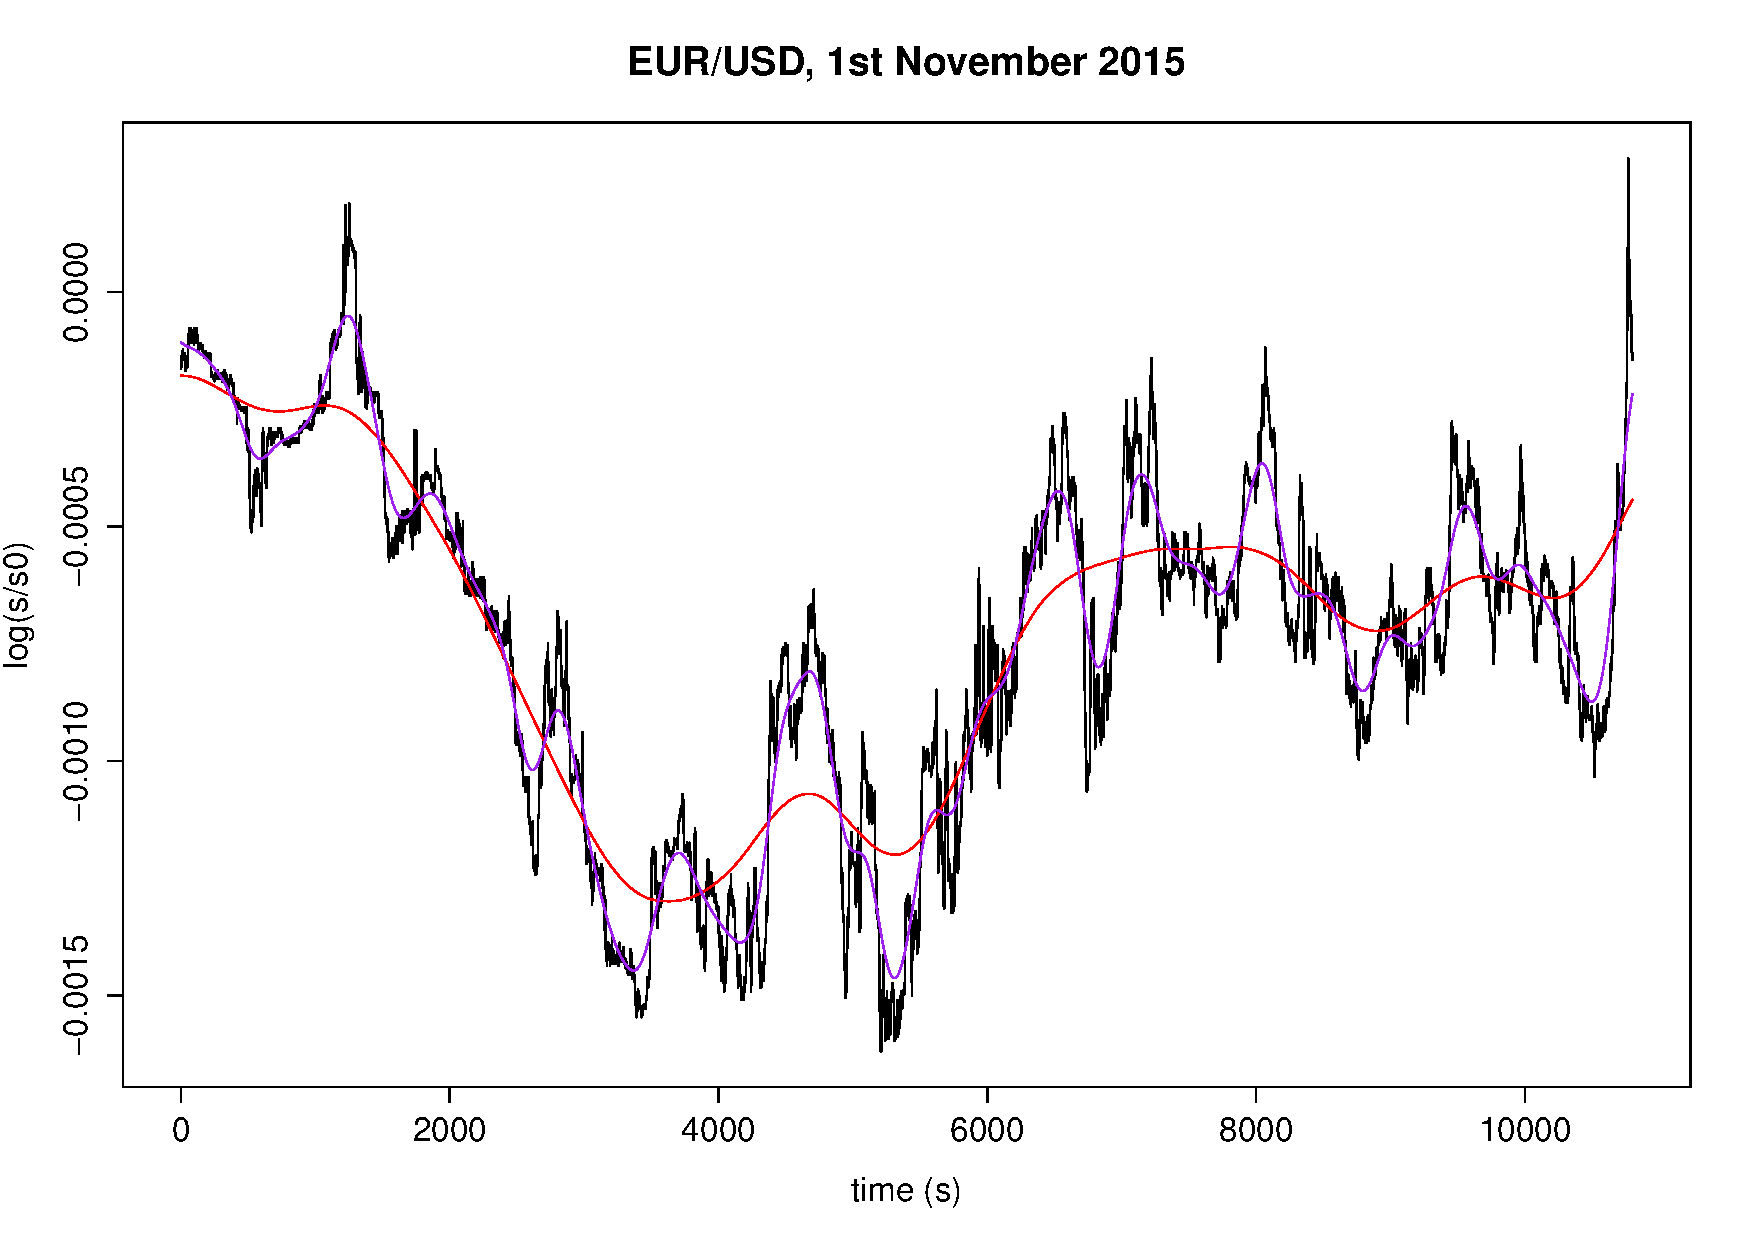
\includegraphics[width=\columnwidth]{figures/asset/ex_filtering}
%\caption{\textbf{Example of the multi-scalar structure of the signal, basis of the construction of synthetic signals | } \emph{Log-prices} are represented on a time window of around 3h for November 1st 2015 for asset EUR/USD, with 10min (purple) and 30min trends.}
%\label{fig:example_signal}
%\end{figure}
%%%%%%%%%%%%%%%%%%%



It is crucial to consider the interference between $\omega_0$ and $\omega_1$ frequencies in the reconstructed signal : correlation indeed estimated is 
\[
\rho_{e} = \rho \left[ \Delta \tilde{X}_1 , \Delta \tilde{X}_2 \right] = \rho \left[ \Delta T_1^{\omega_0} + \Delta \tilde{X}_1^{\omega} , \Delta T_2^{\omega_0} + \Delta \tilde{X}_2^{\omega}\right]
\]
what yields in the reasonable limit $\sigma_1 \gg \sigma_0$ (fundamental frequency small enough), when $\Covb{\Delta \tilde{X}_i^{\omega_1}}{\Delta X_j^{\omega}}=0$ for all $i,j,\omega_1 > \omega$ and returns centered at any scale, the correction on effective correlation due to interferences : we have at first order the expression of effective correlation



\begin{equation}
\label{eq:eff_corr}
\rho_e = \left[ \varepsilon_1 \varepsilon_2 \rho_0 + \rho \right] \cdot \left[ 1 - \frac{1}{2}\left(\varepsilon_1^2 + \varepsilon_2^2 \right) \right]
\end{equation}

{\noindent}what gives the correlation that we can effectively simulate in synthetic data.

Correlation is estimated by Pearson method, with estimator for covariance corrected for bias, i.e.
\[
\hat{\rho}[X1,X2] = \frac{\hat{C}[X1,X2]}{\sqrt{\hat{\Var{}}[X1]\hat{\Var{}}[X2]}}\]
, where $\hat{C}[X1,X2] = \frac{1}{(T-1)}\sum_{t} X_1(t)X_2(t) - \frac{1}{T\cdot (T-1)} \sum_t X_1(t) \sum_t X_2(t)$ and $\hat{\Var{}}[X] = \frac{1}{T}\sum_t{X^2(t)}-\left(\frac{1}{T}\sum_tX(t)\right)^2$.


The tested predictive model $M_{\omega_1}$ is a simple \emph{ARMA} for which parameters $p=2,q=0$ are fixed (as we do not create lagged correlation, we do not expect large orders of auto-regression as these kind of processes have short memory for real data ; furthermore smoothing is not necessary as data are already filtered). It is however applied in an adaptive way\footnote{adaptation level staying low, as parameters $T_W,p,q$ and model type do not vary. We are positioned within the framework of~\cite{potiron2016estimating} which assumes a locally parametric dynamic but for which meta-parameters are fixed. We could imagine a variable $T_W$ which would adapt for the best local fit, the same way parameters are estimated in bayesian signal processing by augmentation of the state with parameters.}. More precisely, given a time window $T_W$, we estimate for any $t$ the model on $[t-T_W+1,t]$ in order to predict signals at $t+1$.



\paragraph{Implementation}

Experiments are implemented in \texttt{R} language, using in particular the \texttt{MTS}~\cite{Tsay:2015xy} library for time-series models. Cleaned data and source code are openly available on the \texttt{git} repository of the project\footnote{at \texttt{https://github.com/JusteRaimbault/SynthAsset}}. 







}

\showmatmethods % Display the Materials and Methods section

\acknow{Please include your acknowledgments here, set in a single paragraph. Please do not include any acknowledgments in the Supporting Information, or anywhere else in the manuscript.}

%\showacknow % Display the acknowledgments section

%\pnasbreak splits and balances the columns before the references.
% If you see unexpected formatting errors, try commenting out this line
% as it can run into problems with floats and footnotes on the final page.
%\pnasbreak

% Bibliography
\bibliography{/Users/Juste/Documents/ComplexSystems/CityNetwork/Biblio/Bibtex/CityNetwork,biblio/biblio}

\end{document}